%%% material_methods.tex --- 

%% Author: garamonfok@gros
%% Version: $Id: material_methods.tex,v 0.0 2011/10/09 18:39:32 garamonfok Exp$

\section{Measuring DNA complexity}
\label{sec:meas-dna-compl}

\subsection{The complexity ratio and complexity value}
\label{sec:compl-ratio-compl}

% \lettrine[lines=4, slope=-0.5em, lhang=0.5, findent=2.1em, nindent=-0.9em, loversize=0.25]{C}{omplexity}
We define the complexity ratio (CR) in terms of classical formulae used in data compression \cite{Adjeroh2008}. Its computation consists of three transformation steps for a given sequence. \textbf{First}, the \mygls{Burrows-Wheeler} transform (BWT) \cite{Burrows1994}, \textbf{second} the Move To Front (MTF) \cite{Ryabko1980} algorithm and, \textbf{finally}, a summary of the unexpected dispersion of the values obtained through Shannon's entropy \cite{Shannon1948} (see \autoref{tab:cr_example} for an example of the process). Thus, the CR is Shannon's entropy of a transformation or digestion of the sequence. The purpose of this transformation is to reveal the regularities in a sequence. Shannon's entropy is zero (i.e. the minimum possible value) only when a sequence consists solely of a single repeated symbol, which is the simplest possible combinatorial structure. Conversely, when entropy is equal to one (the maximum entropy value), it indicates that the sequence has a random-like combinatorial structure. 

\begin{table}[!ht]
  \scriptsize
  \rowcolors{1}{white}{lightgray}
  Given a sequence, $seq=AACCTTCGTAGCATGG$:
  \begin{center}
      \begin{tabular}{clc}
        \hline
        \textbf{\#} & \textbf{Rotating sequence} & \textbf{\textit{I.}} \\ \hline
        0  & AACCTTCGTAGCATG\textbf{G}$|$ & 0  \\
        1  & ACCTTCGTAGCATGG$|$\textbf{A} & 1  \\
        2  & CCTTCGTAGCATGG$|$A\textbf{A} & 5  \\
        3  & CTTCGTAGCATGG$|$AA\textbf{C} & 7  \\
        4  & TTCGTAGCATGG$|$AAC\textbf{C} & 15 \\
        5  & TCGTAGCATGG$|$AACC\textbf{T} & 13 \\
        6  & CGTAGCATGG$|$AACCT\textbf{T} & 6  \\
        7  & GTAGCATGG$|$AACCTT\textbf{C} & 11 \\
        8  & TAGCATGG$|$AACCTTC\textbf{G} & 12 \\
        9  & AGCATGG$|$AACCTTCG\textbf{T} & 2  \\
        10 & GCATGG$|$AACCTTCGT\textbf{A} & 9  \\
        11 & CATGG$|$AACCTTCGTA\textbf{G} & 4  \\
        12 & ATGG$|$AACCTTCGTAG\textbf{C} & 3  \\
        13 & TGG$|$AACCTTCGTAGC\textbf{A} & 14 \\
        14 & GG$|$AACCTTCGTAGCA\textbf{T} & 10 \\
        15 & G$|$AACCTTCGTAGCAT\textbf{G} & 8  \\ \hline
      \end{tabular}
    {\Large\pointer}
      \rowcolors{1}{white}{lightgray}
      \begin{tabular}{ c }
        \hline
        \textbf{BWT} \\ \hline
        G \\
        A \\
        T \\
        C \\
        G \\
        A \\
        T \\
        C \\
        G \\
        A \\
        T \\
        C \\
        G \\
        T \\
        A \\
        C \\ \hline
      \end{tabular}
    {\Large\pointer}
      \rowcolors{1}{white}{lightgray}
      \begin{tabular}{ c c c c c }
        \hline
        \mc{4}{c}{\textbf{Char. list}} & \textbf{MTF} \\ \hline
        \textbf{G} & a & t & c & 0 \\
        G & \textbf{A} & t & c & 1 \\
        A & g & \textbf{T} & c & 2 \\
        T & a & g & \textbf{C} & 3 \\
        C & t & a & \textbf{G} & 3 \\
        G & c & t & \textbf{A} & 3 \\
        A & g & c & \textbf{T} & 3 \\
        T & a & g & \textbf{C} & 3 \\
        C & t & a & \textbf{G} & 3 \\
        G & c & t & \textbf{A} & 3 \\
        A & g & c & \textbf{T} & 3 \\
        T & a & g & \textbf{C} & 3 \\
        C & t & a & \textbf{G} & 3 \\
        G & c & \textbf{T} & a & 2 \\
        T & g & c & \textbf{A} & 3 \\
        A & t & g & \textbf{C} & 3 \\ \hline
      \end{tabular}
  \end{center}
  \pointer 
  $\:\:CR(seq) = E(MTF(BWT(seq))) = E(0, 1, 2, 3, 3, 3, 3, 3, 3, 3, 3, 3, 3, 2, 3, 3) = 0.593$
  \caption [CR explained by an example]{% CORRECTED fill ok with the caption title
    \textbf{CR explained by an example.}\\
    These 3 tables summarize the steps followed to obtain the final sequence of numbers from which Shannon's entropy is computed. 1) The table on the left corresponds to the \mygls{Burrows-Wheeler} transform (BWT). The original sequence is rotated sequentially (so that the first character moves to the back), resulting in different strings and as many strings as characters in the sequence. The resulting sequences are then sorted in lexicographic order. The ``\textit{I.}'' column corresponds to the Index of this ordering (e.g. the sequence number 2 of the original order ``\#'' takes the position 5 in lexicographic order). 2) The table in the center corresponds to the result of the BWT, which comprises the last character of each of the previously ordered sequences. 3) The table on the right corresponds to the application of the MTF algorithm. Starting from a sequence of all characters (named here ``Char. list'' and with four nucleotides in this case), the Move-to-front (MTF) algorithm calculates the index of the BWT nucleotide (upper case bold letter) in the ``Char. list''. In a second step, for the next iteration, MTF transforms the ``Char. list'', bringing to the front the corresponding BWT character (upper case letter). Finally, Shannon's entropy of these latter values is calculated (line below tables), which generates the CR (the CV is obtained by multiplying CR by the length of the sequence).}
  \label{tab:cr_example}
\end{table}

Algorithmically, the BWT of a given sequence summarizes all its lexicographically~-sorted permutations. The MTF transforms a given sequence into a list of numbers. The higher the number, the less the character was used in the previous part of the sequence of length equal to the number of characters found in the sequence (in the case of DNA, this stack contains 4 characters). The MTF operates from left to right. Each generated number is an index in the stack and denotes an alphabetical symbol. Shannon's entropy converts a sequence into a real number between zero and one. It weights the frequency of the alphabetical symbols in a given sequence. For each symbol $i$ in the alphabet, let $p_{(i)}$ be the probability of finding $i$ in the sequence $s$; where $N_i$ is the number of occurrences of $i$ in $s$ and $length(s)$ is the total length of the sequence $s$: 

\begin{equation} \label{eq:prob_seq}
p_{(i)} = \frac {N_i}{length(s)}
\end{equation}

For the  DNA alphabet, entropy is defined as:

\begin{equation} \label{eq:entropy}
E(s) = -\sum_{i=A,C,G,T}p_{(i)} \times log_4(p_{(i)})
\end{equation}

With $i$ being the index of characters used, which for nucleotides ranges from 0 to 3. Thus, the CR can be given as:

\begin{equation} \label{eq:cr}
CR(s) = E(MTF(BWT(s)))
\end{equation}

The complexity value (CV) of a sequence is its CR multiplied by the number of characters in the sequence (here $s$):

\begin{equation} \label{eq:cv}
CV(s) = E(MTF(BWT(s))) \times length(s)
\end{equation}

As the CV of a sequence depends on the transformation of the MTF applied to the entire sequence, sequences can't be split for the analysis.

\subsection{Complexity in strings}
\label{sec:complexity-strings}

\subsubsection{Genomic sequences}
\label{sec:genomic-sequences}

Complete genomes of 54 species were downloaded from the NCBI database resource \cite{Sayers2009} and Ensembl Genome Project \cite{Flicek2011}. Fourteen major groups of taxa were selected: viruses, phages, bacteria, archaea, fungi, amplicomplexa, heterokonta, amebozoa, urochordates, invertebrates, plants, fish, birds, and mammals. Species were chosen based on their interest as model species or the presence of particular biological features such as: variation in genome size, ancestral or recent polyploidy, living in extreme environments, living as intracellular parasites, gene expansion, genome reduction, RNA or single-strand DNA genomes, and synthetic genomes \autoref{tab:genome}. Eukaryote genomes with a coverage of 6$\times$ or greater were chosen. Sexual chromosomes were excluded from the analysis, and ambiguous ``N'' characters were removed from sequences, and thus, excluded when measuring chromosome length. Genome complexity was calculated over concatenated chromosomes.

Complexity in biological sequences was computed in the +1 strand. Analysis of -1 strands did not generate significantly different results.

% CORRECTED ploidy level sound strange -> its ok: http://www.google.com/search?ie=UTF-8&oe=UTF-8&sourceid=navclient&gfns=0&q=%22ploidy+level%22#hl=en&safe=off&sa=X&ei=GCjzT6PsG9S7hAfo3dCmDQ&ved=0CEgQvwUoAA&q=%22with+different+ploidy+level%22&spell=1&bav=on.2,or.r_gc.r_pw.r_qf.,cf.osb&fp=9b0facc6b6dc2725&biw=1280&bih=945
Random sequences with different ploidy levels were also needed for the study and these were generated with the Python base function: ``random'' \cite{VanRossum2003}. The complexity value of biological and random sequences was computed with the DNA alphabet of four letters.

\subsubsection{Annotation of repetitive elements}
\label{sec:annot-repet-elem}

Interspersed repeats and low complexity DNA sequences were screened and mapped in the genomes of all 54 selected species using the RepeatMasker program \cite{Smit2010}. Libraries of genetic elements were retrieved from RepBase (Release 20110419) \cite{Jurka2005}. An example of a summary file generated by RepeatMasker is shown in  \autoref{fig:repe-summ-outp}.

\begin{figure}[!ht]
  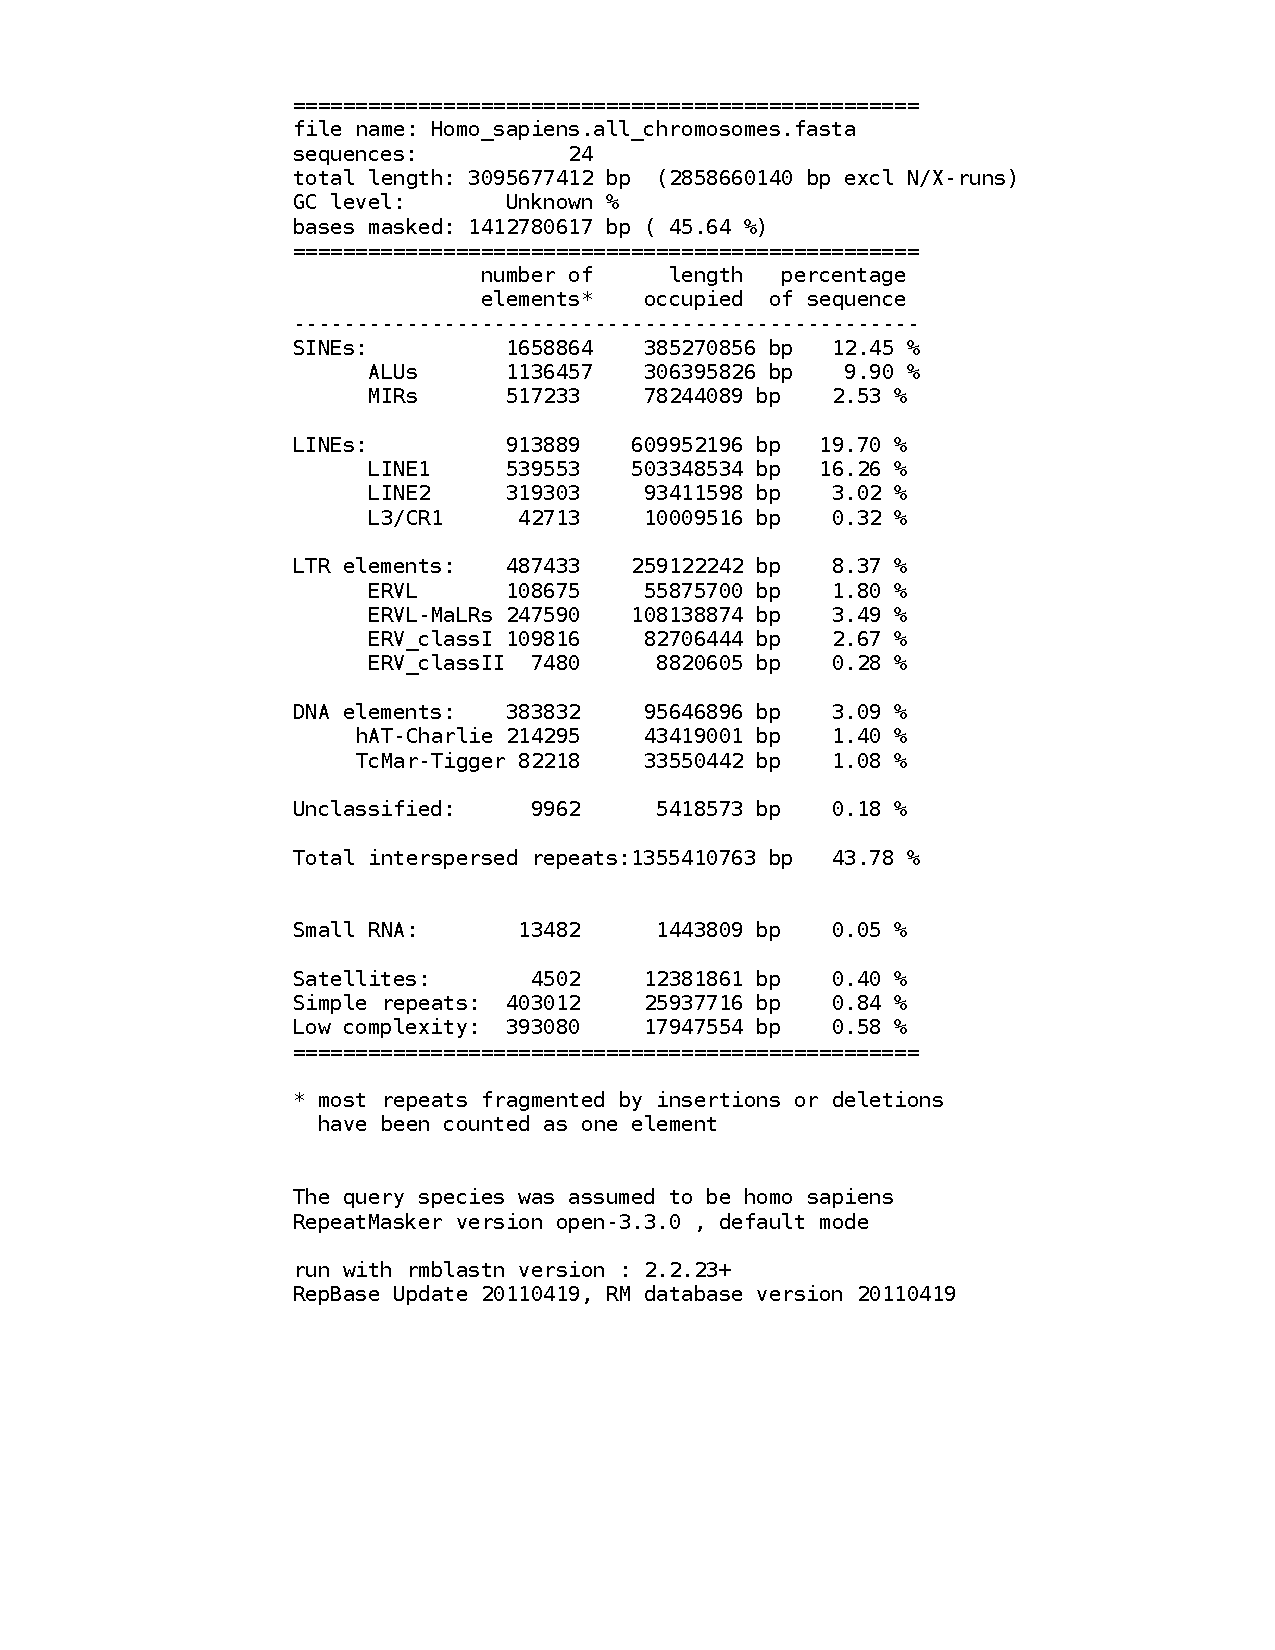
\includegraphics[width=\textwidth,trim=1.5cm 4cm 1.5cm 2cm]{tex_source/Appendix/all_tbl.pdf}
  \caption[RepeatMasker summary output file]{
    \textbf{RepeatMasker summary output file.}\\
    File returned by RepeatMasker for the human genome. It contains the proportion of each family and \mygls{superfamily} of genetic elements found by RepeatMasker, in relation to sequence size (in this case, the entire genome).
  }
  \label{fig:repe-summ-outp}
\end{figure}

The complexity of the major families of repetitive elements such as \myglspl{LTR}, \myglspl{LINE}, \myglspl{SINE}, DNA \myglspl{transposon}, \myglspl{satellite} and exons, introns, and complete genes (considering untranslated regions) was computed after concatenation of all elements but conserving their original order in the chromosomes.

\subsubsection{Human texts}
\label{sec:human-texts}

Short stories, books and complete works in their original languages were downloaded from Project Gutenberg (\myurl{http://www.gutenberg.org/}). To automatically detect the sizes of the alphabets size in texts (including mathematical and punctuation symbols) we run the COMPL program (\myurl{http://kapow.dc.uba.ar/compl}) with the ``auto'' option, that takes into account all characters found, including mathematical symbols, and different punctuation signs. 


% CORRECTED remove this title.... what is windows
\subsubsection{Estimation of complexity in sliding and overlapping windows along chromosomes}
\label{sec:complexity-windows}

To study complexity along chromosomes, a sliding window method that moves along chromosomes in overlapping units of 1.0 Kb to 100 Mb was performed.

% CORRECTED more specific title
\subsection{Simulation of ``polyploid'' random sequence degeneracy through mutation and translocation}
\label{sec:simulations}

We performed four kinds of experiments, in which CV and CR were computed. \textbf{First}: the random polyploid construction of sequences of various sizes and ploidy levels ($1\times$ to $10\times$). \textbf{Second}: evolution over 40 million generations with a constant neutral mutation rate of $1.0e^{-08}$ mutations per site per generation (this value lies between the mutation rate estimated for {\it Homo sapiens}: $2.5e^{-08}$ \cite{Nachman2000} , and \textit{Arabidopsis thaliana}: $7.1e^{-09}$ \cite{Ossowski2010}) for random sequences, and chromosomes of \textit{Zea mays} and \textit{Sorghum bicolor}. \textbf{Third}: evolution over 50,000 generations for random polyploid genomes of different sizes (100Kb, 1Mb, 10Mb) with 1.0 Kb translocations between chromosomes. The number of translocations per generation was set as a constant function of genome size (genome size divided by 1,000). \textbf{Last}: the concatenation and shuffling (computed with the Python base function: ``shuffle'') of all repetition instances in chromosomes for main repetitive families, and genes were considered. The CV and CR values were calculated every 100 generations. 

\section{Measuring dynamics of genetic species}
\label{sec:meas-dynam-genet}

\subsection{Genomes}
\label{sec:genomes}

For the study on the dynamics of genetic elements, the genomic sequences of 31 species from unicellular eukaryotes to mammals were used. These genomes correspond to a subset of the 54 genomes presented in the previous section (see \autoref{sec:complexity-strings}). References can be found in \autoref{tab:genome}, page \pageref{tab:genome}. The complete list of species used is: \begin{inparaenum}[\bgroup\bfseries\em 1\egroup\it)]
\item \textit{Gallus gallus}            (Bird)
\item \textit{Taeniopygia guttata}      (Bird)
\item \textit{Danio rerio}              (Fish)
\item \textit{Oryzias latipes}          (Fish)
\item \textit{Tetraodon nigroviridis}   (Fish)
\item \textit{Saccharomyces cerevisiae} (Fungi)
\item \textit{Anopheles gambiae}        (Invertebrate)
\item \textit{Caenorhabditis elegans}   (Invertebrate)
\item \textit{Drosophila melanogaster}  (Invertebrate)
\item \textit{Tribolium castaneum}      (Invertebrate)
\item \textit{Bos taurus}               (Mammal)
\item \textit{Canis familiaris}         (Mammal)
\item \textit{Equus caballus}           (Mammal)
\item \textit{Homo sapiens}             (Mammal)
\item \textit{Macaca mulatta}           (Mammal)
\item \textit{Monodelphis domestica}    (Mammal)
\item \textit{Mus musculus}             (Mammal)
\item \textit{Pan troglodytes}          (Mammal)
\item \textit{Pongo abelii}             (Mammal)
\item \textit{Rattus norvegicus}        (Mammal)
\item \textit{Arabidopsis lyrata}       (Plant)
\item \textit{Arabidopsis thaliana}     (Plant)
\item \textit{Brachypodium distachyon}  (Plant)
\item \textit{Oryza sativa}             (Plant)
\item \textit{Populus trichocarpa}      (Plant)
\item \textit{Sorghum bicolor}          (Plant)
\item \textit{Zea mays}                 (Plant)
\item \textit{Dictyostelium discoideum} (unicellular Eukaryote)
\item \textit{Plasmodium falciparum}    (unicellular Eukaryote)
\item \textit{Thalassiosira pseudonana} (unicellular Eukaryote)
and \item \textit{Ciona intestinalis}   (Urochordate).
\end{inparaenum}

\subsection{Mining Genetic Species}
\label{sec:mining-genet-elem}

% CORRECTED? the sum... CORRECTED functional elements... \myglspl{biotype}? I think it is ok
For this study, we define genetic species (GSs) as being the aggregate of superfamilies of repetitive elements and functional elements grouped into \myglspl{biotype}, each of which are described below.

\subsubsection{Repetitive Elements}
\label{sec:repetitive-elements}

Repetitive elements were mapped following the methodology explained in \autoref{sec:annot-repet-elem}.

To measure the dynamics of genetic elements, we had to define a level to consider as ``species'' in the RepBase ontology (see \nameref{sec:definition-species}: \autoref{sec:definition-species}). We decided to consider ``species'' as those classes of repeats that can be functionally defined, i.e. corresponding to \myglspl{superfamily} of transposable elements according to \cite{Wicker2007} or, also, to the RepBase classification \cite{Kapitonov2008}.

A complete list of the mapped \myglspl{superfamily} is shown in \autoref{tab:superfamilies}

\begin{table}[ht]
  \scriptsize
  \rowcolors{1}{white}{lightgray}
  \begin{center}
    \begin{tabular*}{\textwidth}{p{0.1504\hsize} p{0.788\hsize} }
      \hline
      \textbf{Family}    & \textbf{\myGlspl{superfamily}}                                                                                                                                                                                                                                                                                                                                                               \\ \hline
      ARTEFACT     & ARTEFACT \\
      DNA          & Academ, Chapaev, Chapaev-Chap3, Crypton, En-Spm, Ginger, Harbinger, Kolobok-Hydra, Kolobok-IS4EU, Kolobok-T2, Maverick, Merlin, Mirage, MuDR, NOF, Novosib, P, PiggyBac, Sola, TcMar, TcMar-Ant1, TcMar-Fot1, TcMar-Gizmo, TcMar-ISRm11, TcMar-Mariner, TcMar-Mogwai, TcMar-Pogo, TcMar-Stowaway, TcMar-Tc1, TcMar-Tc2, TcMar-Tc4, TcMar-Tigger, TcMar-m44, Tourist, Transib, Zator, hAT, hAT-Ac, hAT-Blackjack, hAT-Charlie, hAT-Gulliver, hAT-Pegasus, hAT-Restless, hAT-Tag1, hAT-Tip100, hAT-Tol2, hAT-hAT1, hAT-hAT5, hAT-hATm, hAT-hATw, hAT-hATx, hAT-hobo \\
      \mygls{LINE}         & CR1, CRE, DIRS, DRE, Dong-R4, Genie, I, Jockey, L1, L1-Tx1, L2, L2-Hydra, LOA, Odin, Penelope, Proto1, Proto2, R1, R2, R2-Hero, RTE, RTE-BovB, RTE-RTE, RTE-X, Rex-Babar, Tad1, Zorro, telomeric \\
      \mygls{LTR}          & Caulimovirus, Copia, Copia(Xen1), DIRS, ERV, ERV-Foamy, ERV-Lenti, ERV1, ERVK, ERVL, ERVL-MaLR, Gypsy, Gypsy-Troyka, Ngaro, Pao, TATE, Viper \\
      Low complexity & Low complexity \\
      Other        & Composite, DNA virus, centromeric, subtelomeric \\
      RC           & Helitron \\
      RNA          & RNA \\
      \mygls{SINE}         & 5S, 7SL, Alu, B2, B4, BovA, C, CORE, Deu, Dong-R4, I, ID, L1, L2, MIR, Mermaid, R1, R2, RTE, RTE-BovB, Salmon, Sauria, V, tRNA, tRNA-7SL, tRNA-CR1, tRNA-Glu, tRNA-L2, tRNA-Lys, tRNA-R2, tRNA-RTE \\
      \myGls{satellite}    & W-chromosome, Y-chromosome, acromeric, centromeric, macro, subtelomeric, telomeric \\
      Simple repeat & Simple repeat \\
      Unknown      & Y-chromosome, centromeric \\
      rRNA         & rRNA \\
      scRNA        & scRNA \\
      snRNA        & snRNA \\
      tRNA         & tRNA \\      
      \hline
    \end{tabular*}
    \caption [Superfamily of repetitive elements and description]{%
      \textbf{\myGlspl{superfamily} of repetitive elements and description.}\\
      % CORRECTED:  put -> Complete list of \myglspl{superfamily} of repetitive elements found in ...donde sea usingh Repeat Masker and RepBase family
      Complete list of the \myglspl{superfamily} of repetitive elements mapped by RepeatMasker using the RepBase library (Release 20110419).}
    \label{tab:superfamilies}
  \end{center}
\end{table}

\subsubsection{Functional Elements}
\label{sec:functional-elements}

Functional elements correspond to \myglspl{biotype} categories of the genes according to the Ensembl \cite{Flicek2011} nomenclature. They were retrieved using the Biomart API \cite{Kinsella2011}. The non-redundant list of functional elements across all species is shown in \autoref{tab:biotypes}.

\begin{table}[ht]
  \scriptsize
  \rowcolors{1}{white}{lightgray}
  \begin{center}
    \begin{tabular*}{\textwidth}{p{0.2004\hsize} p{0.738\hsize} }
      \hline
      \textbf{\myGls{biotype}}     & \textbf{Description}                                                                        \\ \hline
      IG C gene            & Immunoglobulin constant segment                                                             \\
      IG D gene            & Immunoglobulin diversity segment                                                            \\
      IG J gene            & Immunoglobulin joining segment                                                              \\
      IG V gene            & Immunoglobulin variable segment                                                             \\
      IG Z gene            & Immunoglobulin gene found in Zebrafish                                                      \\
      MRP RNA              & Mitochondrial RNA-processing RNA                                                            \\
      RNase MRP RNA        & Enzymatically active ribonucleoprotein                                                      \\
      RNase P RNA          & Enzymatically active ribonucleoprotein                                                      \\
      SRP RNA              & Signal recognition particle RNA                                                             \\
      TR C                 & T cell receptor constant domain                                                             \\
      TR J                 & T cell receptor joining domain                                                              \\
      TR V                 & T cell receptor variable domain                                                             \\
      class I RNA          & Class of small non-coding RNA                                                               \\
      class II RNA         & Class of small non-coding RNA                                                               \\
      lincRNA              & Large intervening non-coding RNA (multiexonic non-coding RNA)                               \\
      miRNA                & Micro RNA                                                                                   \\
      misc RNA             & Miscellaneous RNA                                                                           \\
      ncRNA                & Non-coding RNA                                                                              \\
      processed transcript & Non-coding transcript without open reading frame (ORF).                                     \\
      protein coding       & Contains an open reading frame (ORF)                                                        \\
      rRNA                 & Ribosomal RNA                                                                               \\
      retrotransposed      & Non-coding pseudogene produced by integration of a reverse transcribed mRNA into the genome \\
      snRNA                & Small nuclear RNA                                                                           \\
      snlRNA               & Small nuclear like RNA                                                                      \\
      snoRNA               & Small nucleolar RNA, involved in modifications of other RNAs                                \\
      tRNA                 & Transfer RNA                                                                                \\
      transposable element & Transposable element                                                                        \\ \hline
    \end{tabular*}
    \caption [Biotypes and description]{%
      % CORRECTED review this part
      \textbf{\myGls{biotype} and description.} \\
      List of \myglspl{biotype} used a short description retrieved from the Ensembl glossary \cite{Flicek2011} and from the Sequence Ontology browser \cite{Eilbeck2005}.}
    \label{tab:biotypes}
  \end{center}
\end{table}

Note that pseudogenes are not included in this list in order to keep the functional aspect of this category of GSs.

% CORRECTED Random distribution-> title must be more specific
\subsection{Simulated random distribution of genetic elements among chromosomes}
\label{sec:rand-genet-elem}

In order to test for the random distribution of GSs among the chromosomes of each genome, we generated 1,000 genomes corresponding to each species with a random distribution of GSs for each generated genome.

Consequently, the GSs of each genome were distributed among the chromosomes according to a probability dependent on the size of the chromosome. As an example, in the human genome,  it was around six times more likely for a GS to occur in chromosome 1 than chromosome 22 (chromosome lengths were 225 megabases and 35 megabases for chromosome 1 and 22 respectively).

% CORRECTED not well written
Since chromosome size is critical to the randomization process, we decided to remove chromosome regions where no GSs would be found (e.g. centromeric regions or incompletely sequenced regions) from the computation. For this purpose, we  defined chromosome size as being the sum of all 10 kilobase regions containing at least one GS (see \autoref{tab:example_chrom_size}).


\rowcolors{1}{white}{lightgray}
\begin{table}[!ht]
  \scriptsize
  \begin{center}
    \begin{tabular}{ r r r r }
      \hline
      \textbf{Chromosome} & \textbf{Chromosome length} & \textbf{Corrected length} & \textbf{Percentage remaining} \\ \hline
      1            & 249,240,621         & 225,200,000               & 90.35\%                  \\
      2            & 243,188,741         & 237,670,000               & 97.73\%                  \\
%      3            & 197,961,181         & 194,230,000               & 98.12\%                  \\
%      4            & 191,044,271         & 187,270,000               & 98.02\%                  \\
%      5            & 180,901,928         & 177,090,000               & 97.89\%                  \\
      6            & 171,048,878         & 167,050,000               & 97.66\%                  \\
%      7            & 159,128,663         & 154,640,000               & 97.18\%                  \\
%      8            & 146,302,151         & 142,290,000               & 97.26\%                  \\
%      9            & 141,151,937         & 120,130,000               & 85.11\%                  \\
      10           & 135,524,747         & 131,040,000               & 96.69\%                  \\
%      11           & 134,946,516         & 130,310,000               & 96.56\%                  \\
      12           & 133,841,891         & 129,970,000               & 97.11\%                  \\
%      13           & 115,109,733         & 95,500,000                & 82.96\%                  \\
%      14           & 107,289,415         & 87,910,000                & 81.94\%                  \\
      15           & 102,521,389         & 81,520,000                & 79.52\%                  \\
%      16           & 90,290,985          & 78,640,000                & 87.10\%                  \\
%      17           & 81,195,208          & 77,700,000                & 95.70\%                  \\
%      18           & 78,017,245          & 74,580,000                & 95.59\%                  \\
%      19           & 59,118,983          & 55,460,000                & 93.81\%                  \\
      20           & 62,962,324          & 59,430,000                & 94.39\%                  \\
%      21           & 48,119,895          & 35,100,000                & 72.94\%                  \\
      22           & 51,244,541          & 34,790,000                & 67.89\%                  \\
      X            & 155,260,558         & 150,230,000               & 96.76\%                  \\
      Y            & 59,033,288          & 22,520,000                & 38.15\%                  \\ \hline
    \end{tabular}
  \end{center}
  \caption[A sample of human chromosome size changes after removing regions without genetic elements (GEs)]{\textbf{A sample of human chromosome size changes after removing regions without genetic elements (GEs).}}
  \label{tab:example_chrom_size}
\end{table}


\subsection{Fitting Neutral Ecological models}
\label{sec:neutr-ecol-models}

\subsubsection{Ewens sampling formula}
\label{sec:ewens-model}

Ewens sampling formula \cite{Ewens1972} (\autoref{eq:ewens}) was originally designed in order to describe the number of different alleles expected to be observed in a given sample. However, the formula can be applied to other scientific fields. In the context of the study of ecological communities, its application was first suggested  by Tavar\'e and Ewens \cite{Tavari1997} and finally implemented by Hubbell \cite{Hubbell2001}. Hubbell proposed a model that defined the fundamental biodiversity parameter $\theta$ (\autoref{eq:theta}), given the speciation rate $\nu$ and $J_M$ as the size of the metacommunity.

\begin{equation} \label{eq:theta}
\theta = 2J_M\nu
\end{equation}

The estimation of $\theta$ alone is sufficient to directly apply Ewens sampling formula (\autoref{eq:ewens}), and to compute its likelihood for given a community (\autoref{eq:ewens_lnl}).

\begin{equation} \label{eq:ewens}
Pr\{S,n1,n2,\ldots,n_S|\theta\} = \frac{J_M!\theta^S}{1^{\phi1} 2^{\phi2} \cdots J_M^{\phi J_M} \phi_1! \phi_2! \cdots \phi_{J_M}! \prod_{k=1}^{J_M} (\theta + k - 1)}
\end{equation}

Here $n_i$ corresponds to the abundance of species $i$, and $\phi_a$ the number of species with abundance $a$.

\begin{equation} \label{eq:ewens_lnl}
\mathcal{L} = \frac{\theta^S}{\prod_{k=1}^{J_M} (\theta + k - 1)}
\end{equation}

\subsubsection{Etienne's sampling formula}
\label{sec:etienne-model}

The main problem with Hubbell's model using Ewens sampling formula is the assumption that migration is unlimited ($m=1$). However a new sampling formula was presented recently \cite{Etienne2005}, which includes cases of $m<1$, taking into account the number of immigrants $I$ depending on the sample size $J$:

\begin{equation} \label{eq:m}
m = \frac{I}{I+J-1}
\end{equation}

Etienne's sampling formula is then postulated as:

\begin{equation} \label{eq:etienne_lnl}
P[D|\theta,m,J] = \frac{J!}{\prod_{i=1}^Sn_i \prod_{j=1}^J\phi_J!} \frac{\theta^S}{(I)_J} \sum_{A=S}^JK(D,A) \frac{I^A}{(\theta)_A}
\end{equation}

with $K(D,A)$ as:

\begin{equation} \label{eq:kda}
K(D,A) := \sum_{\{a_1,\ldots,a_s|\sum_{i=1}^Sa_i=A\}}\prod_{i=1}^S\frac{\bar{s}(n_i,a_i)\bar{s}(a_i,1)}{\bar{s}(n_i,1)}
\end{equation}

Once $K(D,A)$ has been computed, the likelihood of the model can be optimized (\autoref{eq:etienne_lnl}) by varying the values of the parameters $\theta$ and $m$ (see \nameref{sec:model-optimization} \autoref{sec:model-optimization}) for a given dataset.

%This last step is actually the main computational bottle neck in the resolution of Etienne's formula (\autoref{eq:etienne_lnl}), and in particular the calculation the stirling numbers \cite{Etienne2005} in $K(D,A)$'s equation (see \autoref{eq:kda}). A solution was given by Franck Jabot and J\'er\^ome Chave \cite{Jabot2008} and implemented in the Tetame program. It consists in taking advantage of the recurrence function (\autoref{eq:stirling_req}), that allows to build a table of values, given the dispersion of the ranked abundance of species, instead of computing them directly for each pair of values.

%\begin{equation} \label{eq:stirling_req}
%S_{(n,m)} = S_{(n-1, m-1)} - (n-1) \times S_{(n-1, m)}
%\end{equation}

%However, at the expense of the amelioration in computation time, the size of the table of values created using this methodology was excessive in the case of genomic data. A solution, implemented in Ecolopy, was to recursively remove the stirling numbers not needed for the estimation of the $K(D,A)$.

%Finally, given the order of magnitude that can reach the values of stirling numbers ($>1e^{+1000}$ for medium size chromosomes), we needed to discard mathematics operations provided in Python. To be able to deal with this kind of data Ecolopy uses the GMP \cite{Granlund2000} and MPFR \cite{Fousse2007} libraries through GMPY biding \cite{Martelli2007}.

\subsection{Model optimization}
\label{sec:model-optimization}

Models where optimized using different optimization strategies depending on the model selected. In the case of Ewens formula, $\theta$ is the only parameter taken into account, and its estimation is achieved with a single optimization step. For Etienne's model, two parameters were optimized, $\theta$ and $m$, using the best solution of different optimization strategies (see chapter \textbf{\nameref{sec:ecolopy}}, page \pageref{sec:ecolopy} for more details).

A way to ensure that the optimized parameters of Etienne's model truly point to the maximum likelihood consists of placing them over a likelihood surface corresponding to a range of  $\theta$ and $m$ values. The computation time needed to generate such likelihood contour plots prevented its application to all chromosomes in the dataset. Nevertheless, for the five chromosomes tested, the optimal values of $\theta$ and $m$ visually represented in the contour plots were congruent with the results of the optimization (see \autoref{fig:lnl_chrom} as an example of this validation step).

\begin{figure}[!ht]
\centering 
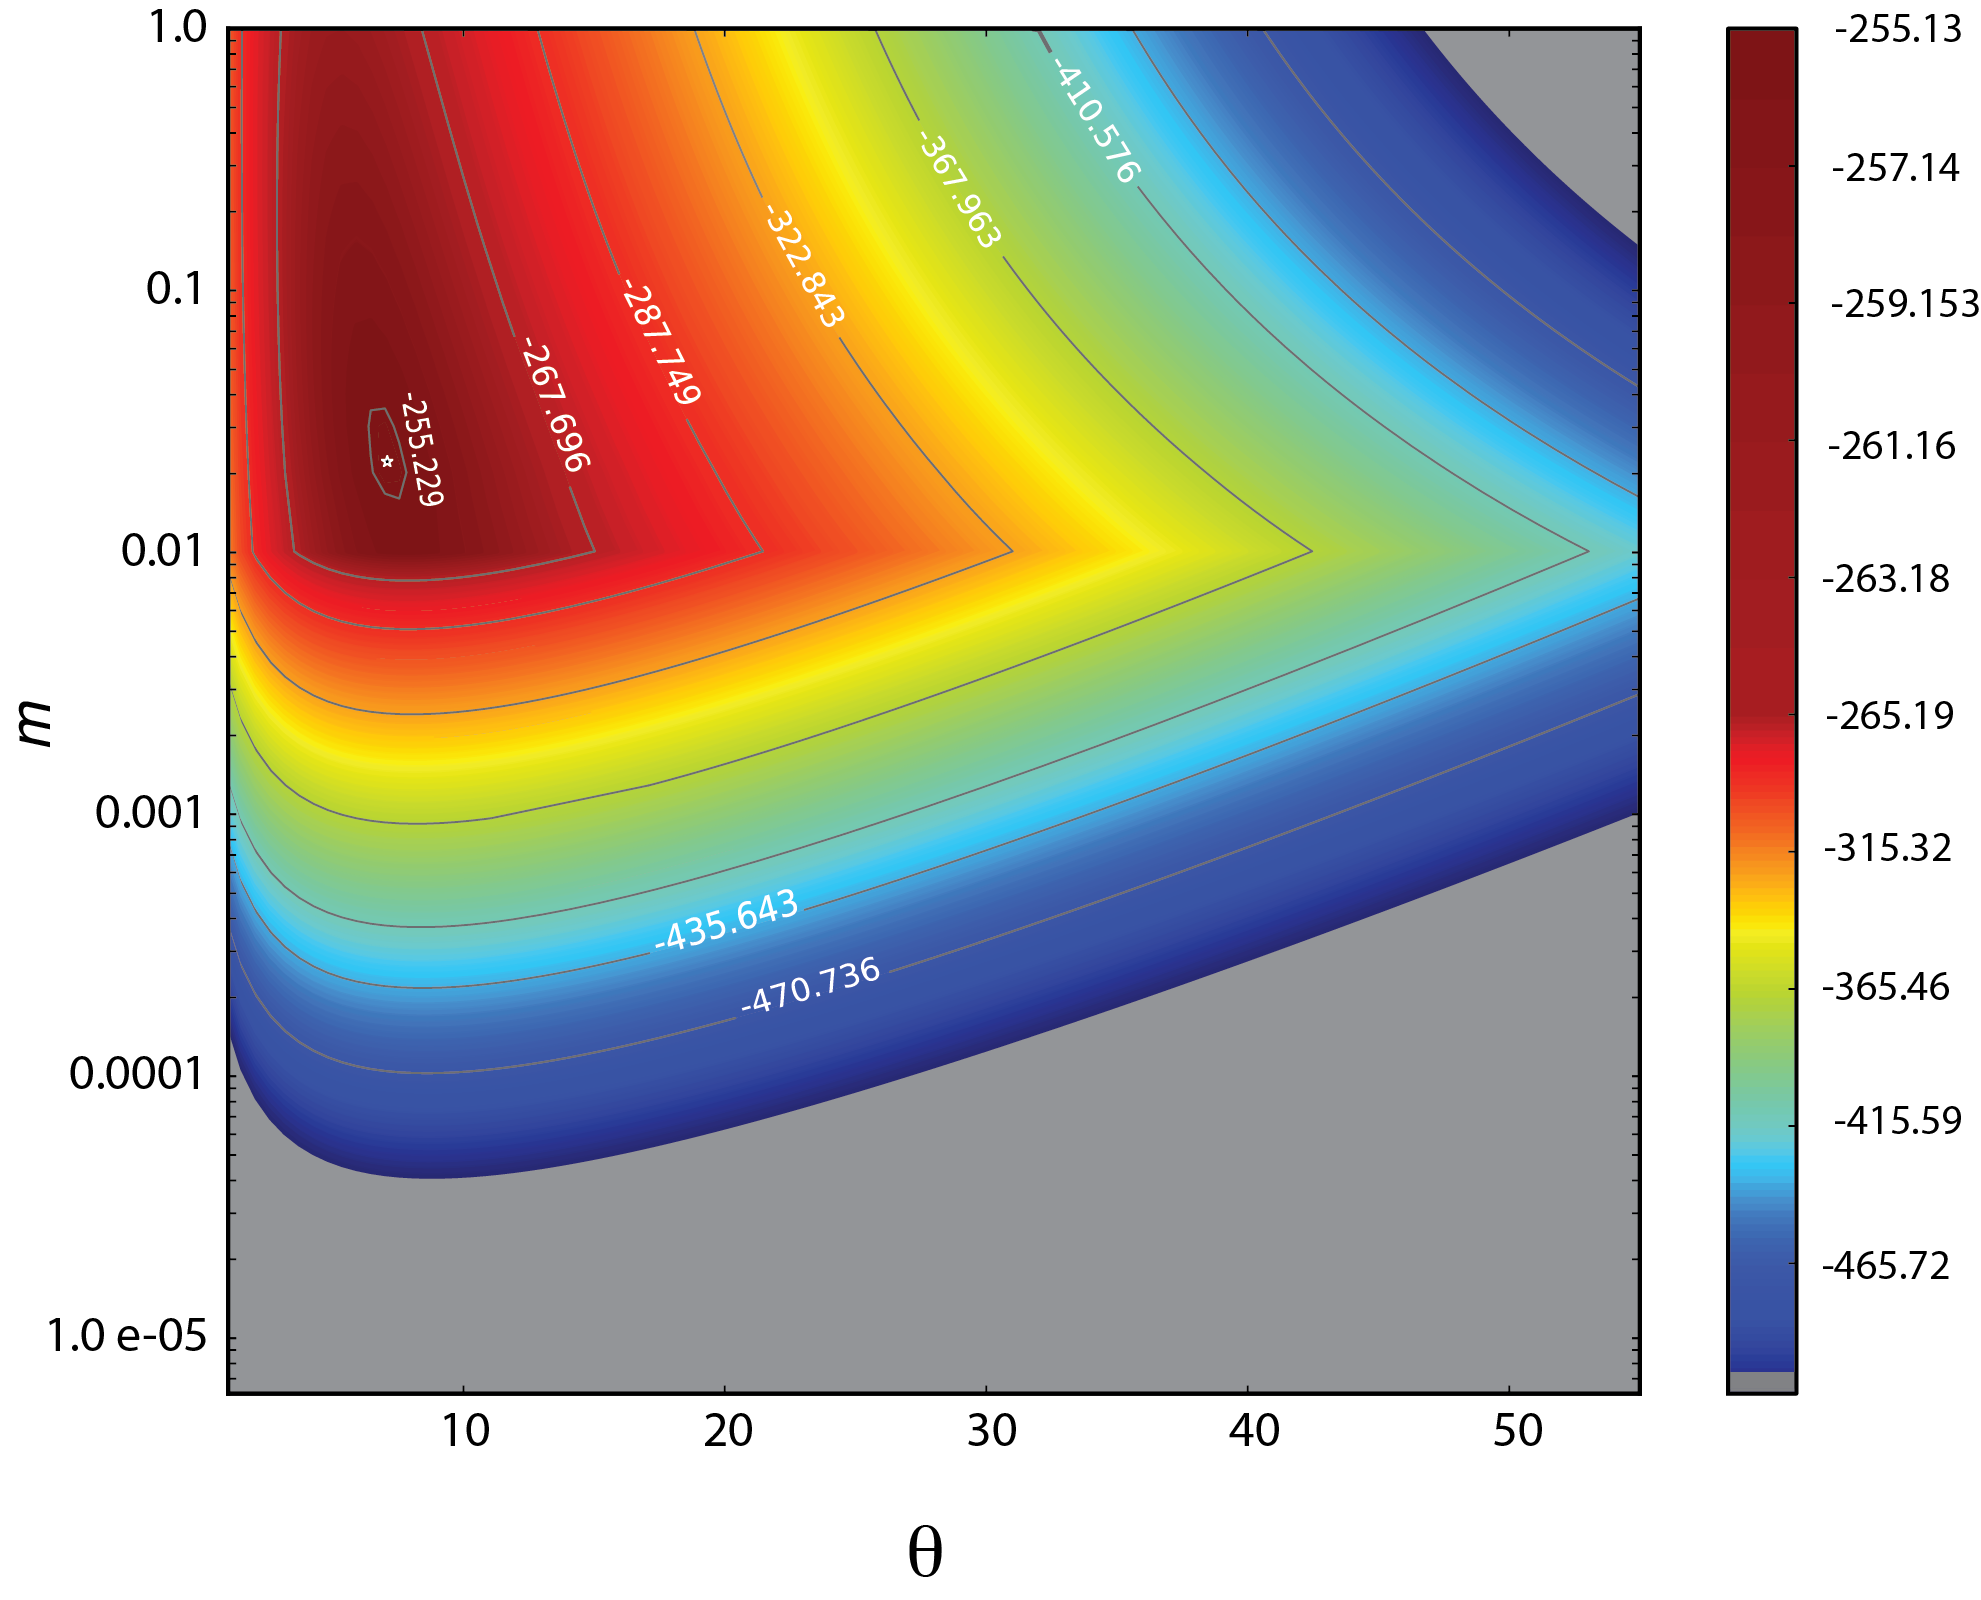
\includegraphics[width=0.95\textwidth]{figures/material_methods/lnl_chrom.png}
\caption[Maximum likelihood inference of neutral parameters]{
  {\bf Maximum likelihood inference of neutral parameters.}\\
  Log likelihood surface as a function of the migration rate ($m$), and the fundamental biodiversity number ($\theta$) for \textit{D. rerio} chromosome 19. Dark red color shows regions of the surface where parameters maximize the probability of explaining the abundance and diversity of observed genetic elements in the chromosome. Likelihood-ratio tests favored Etienne's sampling formula over that of Ewens to explain the observed data in the chromosome.}
\label{fig:lnl_chrom}
\end{figure}

\subsection{Model testing -- Likelihood-ratio test}
\label{sec:model-test-likel}

% CORRECTED check likelihood-ratio test/likelihood-ratio-test
In order to compare and test the fit of a given distribution in the two models computed, a likelihood-ratio test \cite{Wilks1938} can be conducted between them. Etienne's model has two free parameters ($FP$) while Ewens' model only has one. Thus, the number of degrees of freedom for the chi-squared distribution is 1 ($df=FP_{Etienne}-FP_{Ewens}=1$).

\subsection{Testing UNTB}
\label{sec:testing-untb}

In recent years, at least two tests have been developed in order to accept or reject the neutrality of a given ecological community. Both these tests are based on the comparison of a given number of random neutral communities (or replicates) to the observed distribution of abundances. Since replicates are generated using the parameters estimated (see \autoref{sec:model-optimization}) for the real data under a given neutral model (either Ewens or Etienne's model), we expected that they would be very close to the original distribution of abundances. The distances between replicates and the original data is thus a measure of how well the data fits a neutral model.

The first test \cite{Etienne2007} consists of comparing the likelihoods of data fitting the neutral model. Random neutral abundances are fitted to the model, and their likelihoods are used to build a distribution of values. Then, this distribution is compared to the likelihood of the real data. The major problem with this test is technical; the computation time needed to optimize the parameters of each simulated distribution is unrealistically high when dealing with genomic data.

The second test \cite{Jabot2011} uses, instead of likelihood, the comparison of Shannon's entropy \cite{Shannon1948} of each distribution of abundances. It is much faster as replicates do not need to be fitted to a neutral model.

Due to the extent of the dataset in this study, the results presented here are generated from the comparison of Shannon's entropies.

From the neutral parameters obtained for each chromosome, we simulated 10,000 replicates and computed, for each, their Shannon's entropy ($H$). Chromosomes were considered significantly non-neutral when the $H$ of their abundances was below 95\% of the 10,000 simulated $H$ values. \autoref{fig:shannon_distrib} shows the distribution of $H$ for 10,000 simulations under Etienne's model with $S$, $J$ fixed for the observed numbers and $\theta$ and $m$ corresponding to optimized values for two chromosomes.

\begin{figure}[!ht]
  \centering
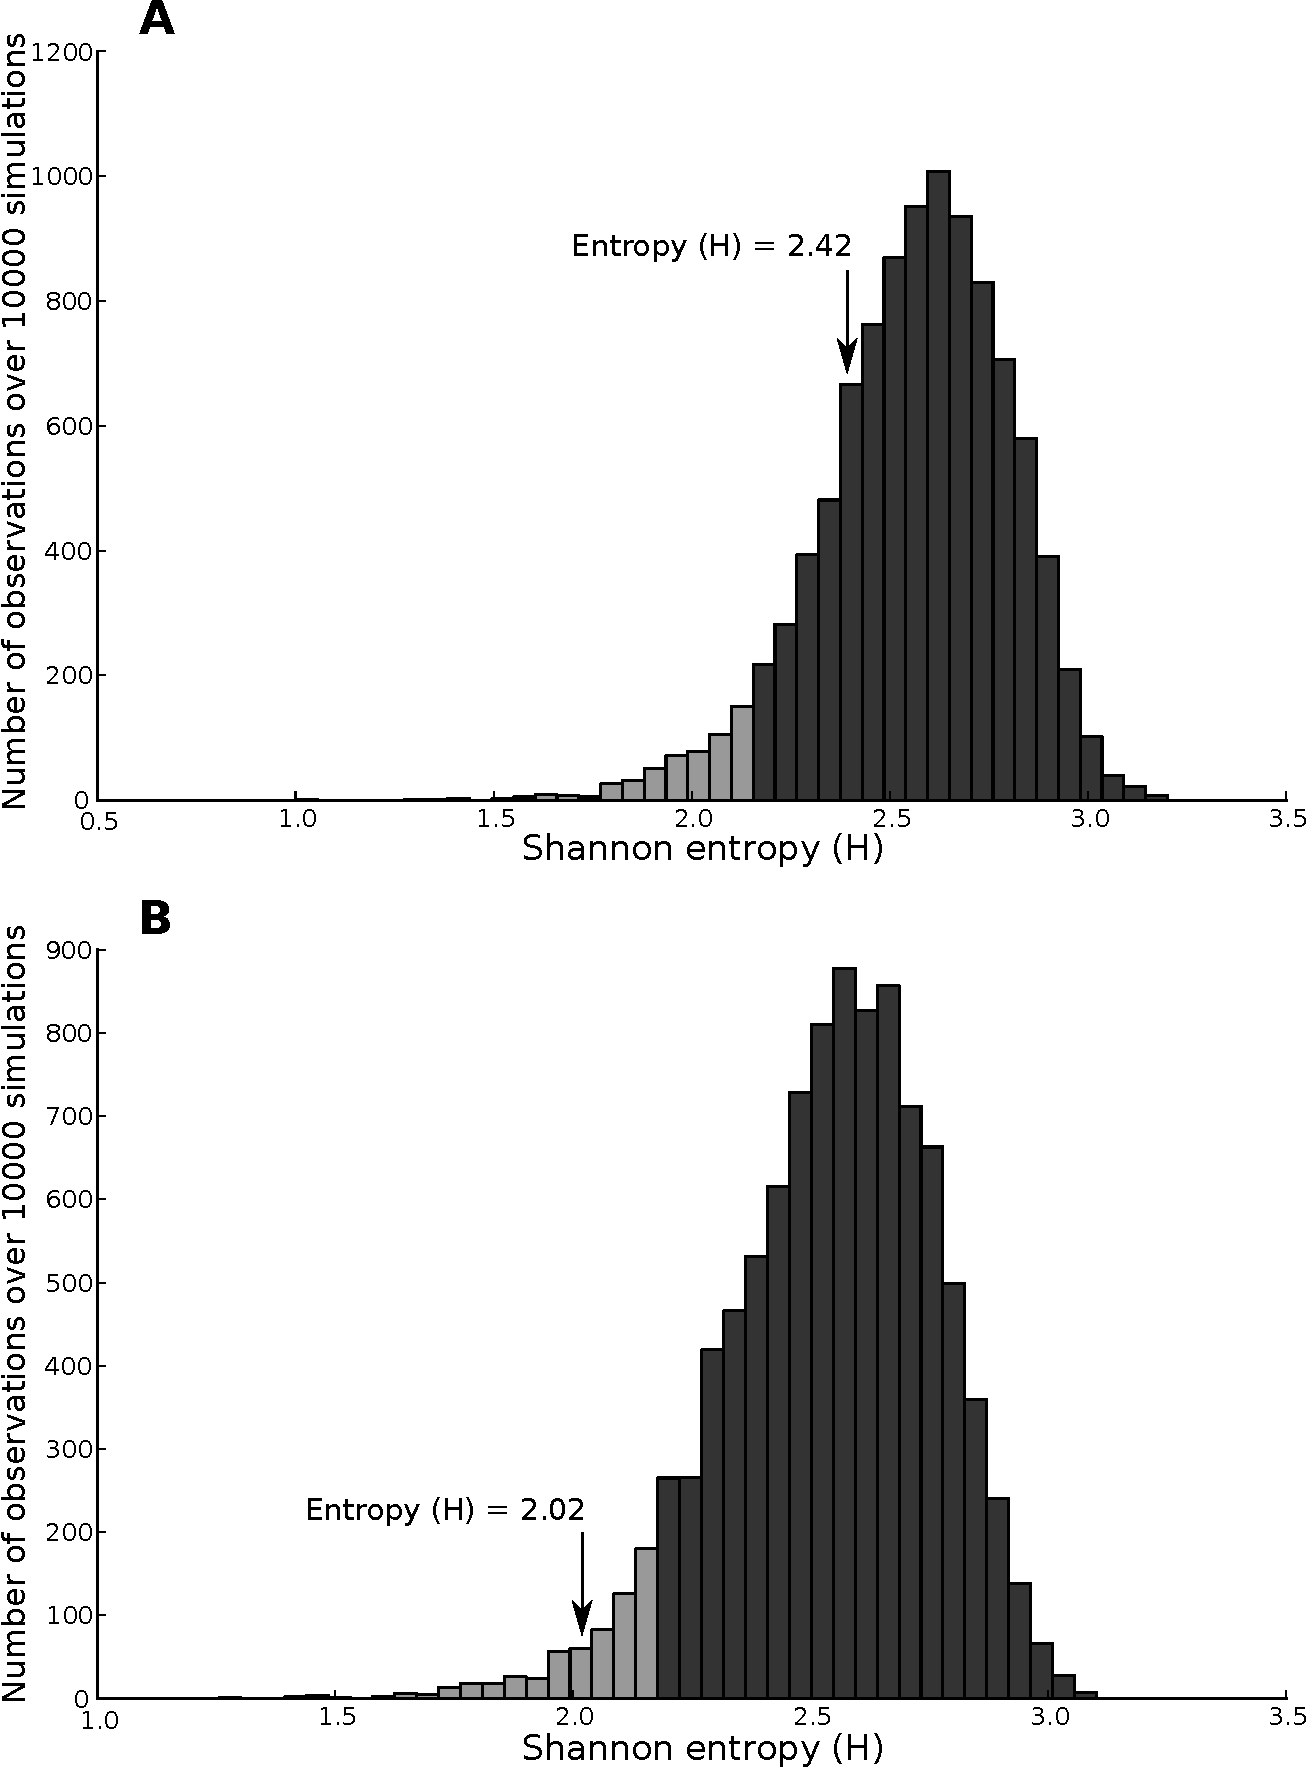
\includegraphics[width=0.74\textwidth]{figures/material_methods/shannon_distr_hsap_chr1_agam_chr2L.pdf}
\caption[Comparing simulated and empirical evenness]{
  {\bf Comparing simulated and empirical evenness. }\\
  The neutrality test compares simulated null distribution of $H$ with the empirical value. The null distribution of $H$ values corresponds to 10,000 neutral simulations of (A) \textit{H. sapiens} chromosome 1 and (B) \textit{A. gambiae} chromosome 2L, with parameters ($\theta$ and $m$) optimized according to Etienne's model. Light and dark gray bars display 5\% and 95\% of the simulated data, respectively. Although neutrality was not rejected in \textbf{B} (p=0.291 and p=0.041 for \textbf{A} and \textbf{B} respectively), posterior correction by multiple testing favored the neutral hypothesis in both cases (q=0.609 and q=0.159 for \textbf{A} and \textbf{B} respectively).}
  \label{fig:shannon_distrib}
\end{figure}

Additionally, given the large number of test performed (one for each of the 548 chromosomes), we corrected statistical significances by the false discovery rate (FDR) method \cite{Benjamini2001}. In \fref{fig:shannon_distrib}{B}, chromosome 2L of \textit{Anopheles gambiae's} is deemed neutral only after correction by FDR.

Given the lack of differences among the results presented in section: \textbf{\nameref{sec:neutrality-sad}} (page \pageref{sec:neutrality-sad}), we replicated this test and fixed the number of species (S) to the observed values in chromosomes. No differences were observed in relation to the number of chromosomes that fitted neutral models.

\subsubsection{Power and specificity of the neutral test}
\label{sec:power-spec-neutr}
% CORRECTED is it really type I and type II error? -> ok Type I: false positive, Type II: false negative
\begin{PPfigure}
  \qquad
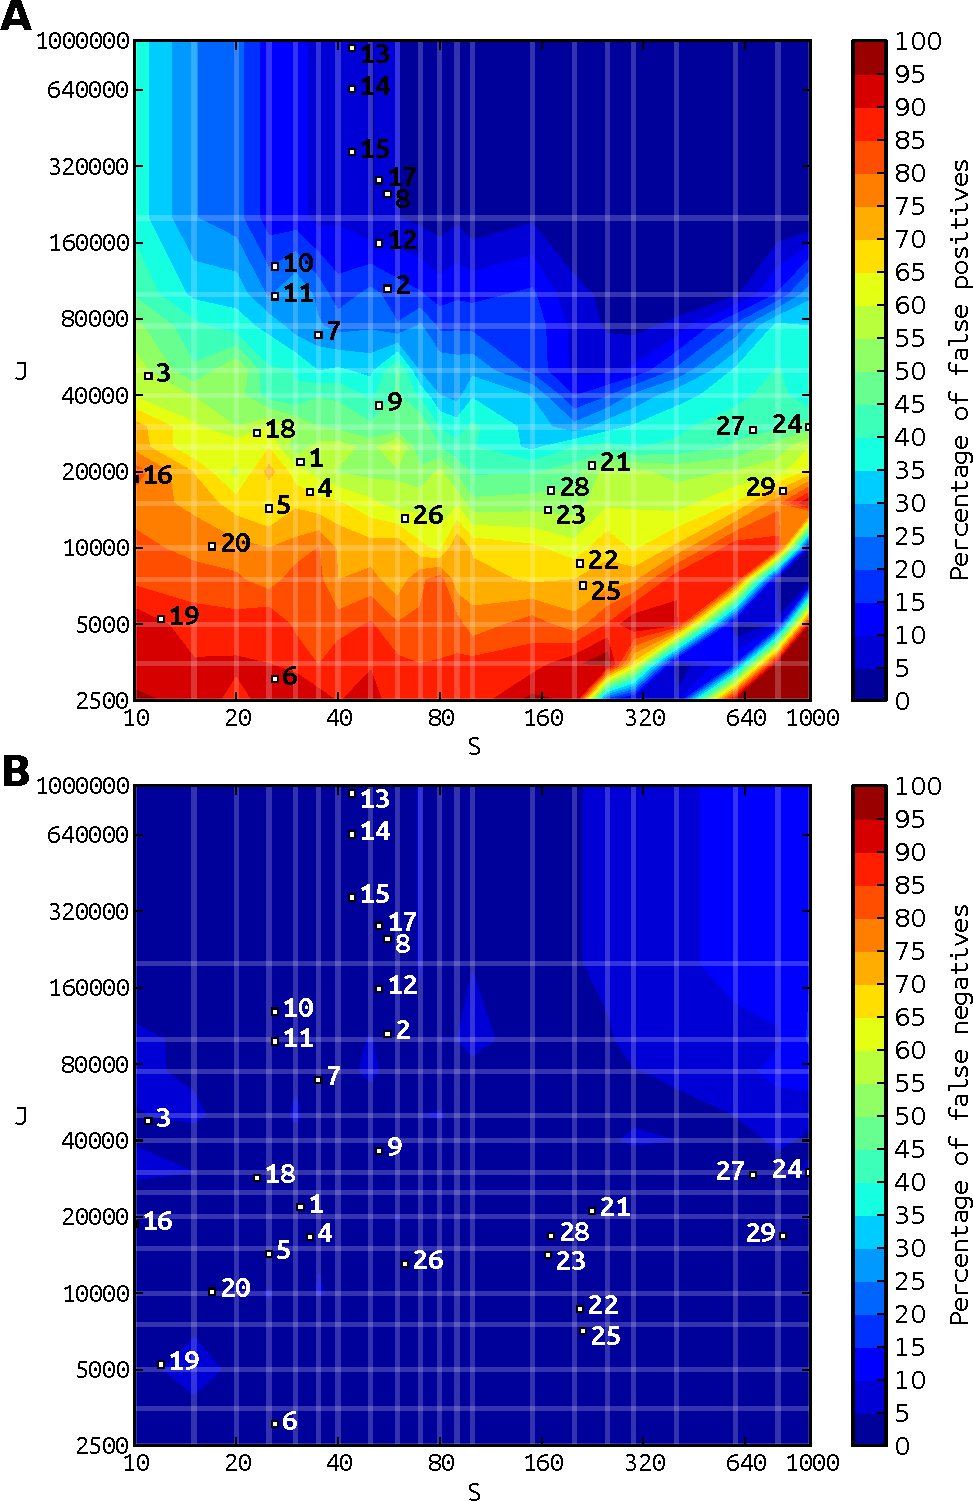
\includegraphics[height=.9\textheight]{figures/material_methods/power_and_sensitivity_test.pdf}
\caption[Type I and Type II errors of the neutral test in ranges of \textit{S} and \textit{J}]{
  {\bf Type I and Type II errors of the neutral test in ranges of \textit{S} and \textit{J}.}\\
  Panels describe the proportion of times the test (\textbf{A}) rejected the null hypothesis when it was true (red regions indicating areas prone to Type I error), and (\textbf{B}) failed to reject the null hypothesis when it was false (light blue regions indicating areas more prone to Type II error). The numbers in both panels are chromosomes:
  \textbf{1}- \textit{A. thaliana} chr1;
  \textbf{2}- \textit{D.rerio} chr1;
  \textbf{3}- \textit{D.discoideum} chr2;
  \textbf{4}- \textit{C.elegans} chrI;
  \textbf{5}- \textit{D.melanogaster} chr2L;
  \textbf{6}- \textit{G.gallus} chr8;
  \textbf{7}- \textit{G.gallus} chr2;
  \textbf{8}- \textit{H.sapiens} chr1;
  \textbf{9}- \textit{H.sapiens} chr1;
  \textbf{10}- \textit{Z.mays} chr1;
  \textbf{11}- \textit{Z.mays} chr3;
  \textbf{12}- \textit{M.musculus} chr0;
  \textbf{13}- \textit{M.domesticus} chr1;
  \textbf{14}- \textit{M.domesticus} chr3;
  \textbf{15}- \textit{M.domesticus} chr5;
  \textbf{16}- \textit{P.falciparum} chr3;
  \textbf{17}- \textit{R.norvegicus} chr1;
  \textbf{18}- \textit{S.bicolor} chr7;
  \textbf{19}- \textit{T.nigroviridis} chr9;
  \textbf{20}- \textit{T.castaneum} chr8; and ecosystems \cite{Jabot2011}:
  \textbf{21}- BCI;
  \textbf{22}- Edoro;
  \textbf{23}- La Planada;
  \textbf{24}- Lambir;
  \textbf{25}- Lenda;
  \textbf{26}- Mudamalai;
  \textbf{27}- Pasoh;
  \textbf{28}- Sinharaja;
  \textbf{29}- Yasuni.}
  \label{fig:power-spec-neutr}
\end{PPfigure}

In order to validate the test of neutrality, we computed the proportion of false and true positives by generating, respectively, random log-normal distributions and random neutral distributions. The results of the test of neutrality applied over log-normal or neutral random distributions are shown in \autoref{fig:power-spec-neutr} panel \textbf{A} and \textbf{B}, respectively.

Accordingly, we can validate the the results given that, in the entire range of $S$ and $J$ values, the proportion of true positives was very high (\fref{fig:power-spec-neutr}{B}. Nevertheless these simulations highlighted some difficulties in differentiating log-normal distributions from neutral distributions. Specifically, when $J<100,000$ individuals, the proportion of false positives is higher than 50\%. However, we decided to overlook this as the increase in the false positive rate only affects the smallest chromosomes, and also because the log-normal distributions used here as alternatives, are known to be barely distinguishable from neutral distributions \cite{McGill2006}.

\section{Selective pressure at molecular level}
\label{sec:gssa_mat-met}

\subsection{Orthology prediction}
\label{sec:orthology-prediction}

The complete genomes of five mammal species (\textit{Homo sapiens}, \textit{Pan troglodytes}, \textit{Mus musculus}, \textit{Rattus norvegicus} and \textit{Canis familiaris}) were retrieved from Ensembl \cite{Flicek2011}. Orthology predictions between \mygls{seed} genes and genes from other species (the \mygls{seed} species was \textit{H. sapiens} in the case of mammals)  were retrieved from Ensembl Compara \cite{Vilella2009} using Biomart \cite{Kinsella2011} (see \autoref{fig:phylogeny} to have an insight of the phylogenies and distances). Of the 23,438 \mygls{seed} genes, only groups of orthologs annotated as ``one-to-one'', i.e. with only one representative of each species, were kept in the final dataset.

\begin{figure}[!ht] 
\centering 
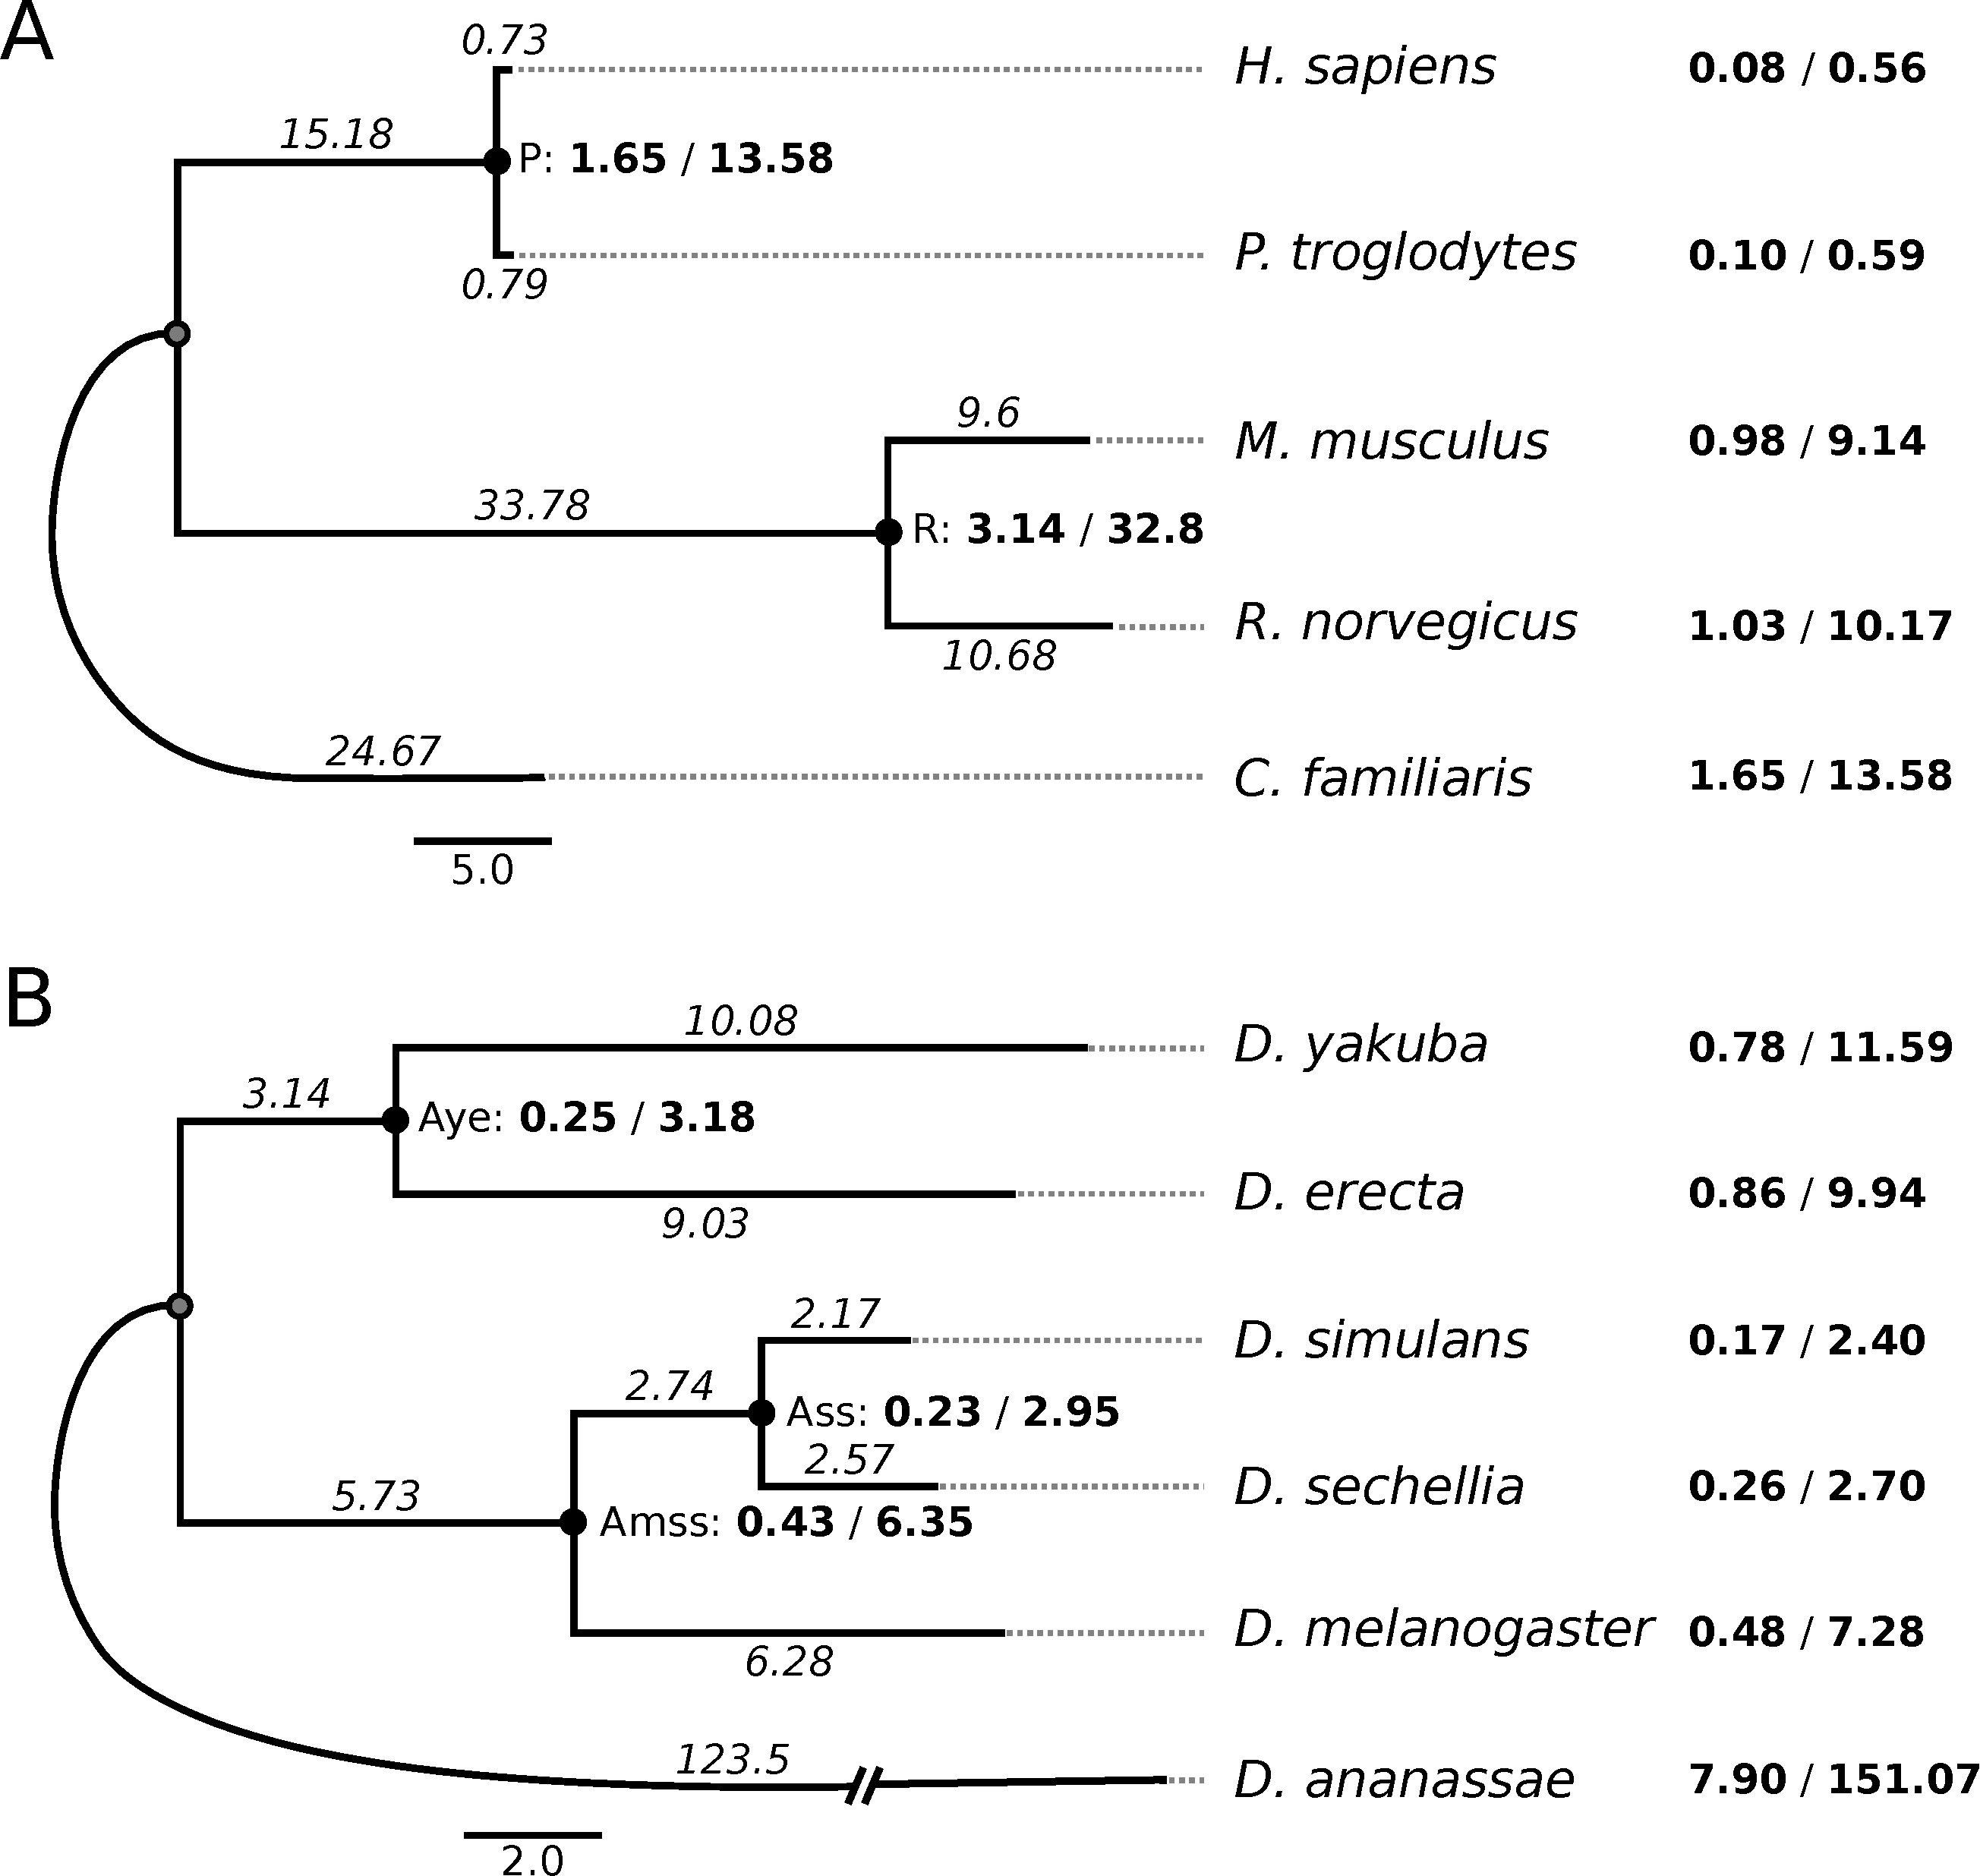
\includegraphics[width=0.85\textwidth]{figures/material_methods/phylogenies.pdf}
\caption[Phylogenies of mammals and species of the \textit{melanogaster} group of \textit{Drosophila}]{
  {\bf Phylogenies of mammals and species of the \textit{melanogaster} group of \textit{Drosophila}.}\\ % CORRECTED no mention about italic numbers... CORRECTED figure confusion italic/straight
  Bold numbers represent the median rates of non-synonymous and synonymous substitutions ($dN$/$dS$) estimated from all coding sequences compared in mammals (\textbf{A}) and \textit{Drosophila} (\textbf{B}). Numbers in italics are median branch lengths. Branch lengths and rates were multiplied by 100. Ancestral estimations were done in primates (P), rodents (R), \textit{D. yakuba} and \textit{D. erecta} (Aye), \textit{D. simulans} and \textit{D. sechellia} (Ass), and \textit{D. melanogaster}, \textit{D. simulans} and \textit{D. sechellia} (Amss). \textit{C. familiaris} in (\textbf{A}), and \textit{D. ananassae} in (\textbf{B}), were chosen as outgroup species.} 
\label{fig:phylogeny}
\end{figure}

The same procedure was applied in six species of \textit{Drosophila}; namely \textit{D. melanogaster} as \mygls{seed}-species, \textit{D. sechellia}, \textit{D. simulans}, \textit{D. yakuba} and \textit{D. erecta} with \textit{D. ananassae} as the outgroup (see \fref{fig:phylogeny}{-B}). Here, the starting number of \mygls{seed} genes was 14,076.
% CORRECTED ok with "was"

\subsection{Alignments, refinement and filters}
\label{sec:alignm-refin-filt}

DNA coding sequences (CDS) were aligned according to the protein translation pattern using Muscle version 3.7 \cite{Edgar2004}, embedded into the CDS-Protal utility in Phylemon 2.0 \cite{Sanchez2011} (see appendix section: \textbf{\nameref{sec:alignment}} at page \pageref{sec:alignment}). Poorly aligned regions were removed using TrimAl \cite{Capella-Gutierrez2009} keeping all sequences but checking the quality of alignment columns with the heuristic method ``-automated-1''. Additionally, alignments smaller than 100 bp were excluded from the analysis.

In mammals, the upper limit for $dN$ and $dS$ considered were those of the human interferon $\gamma$ ($dN = 3.06$) and the relaxin protein \cite{Graur2000} ($dS = 6.39$ substitutions per site per $1e^{+09}$ years). Assuming the human-mouse, mouse-rat and human-chimp speciation times to be about 80, 70 and 5 million years \cite{BlairHedges2003} respectively, orthologous comparisons between primates and rodents with $dS\ge$1 and $dN\ge$0.5, between rodents with $dS\ge$0.256 and  $dN\ge$0.122, and between primates with $dS\ge$0.064 and $dN\ge$0.030 substitutions per site were excluded.

In \textit{Drosophila}, genes were also filtered by high $dN$ and $dS$ values using the fast evolving gene \textit{1G5} as a relaxed reference for both $dN$ and $dS$ \cite{Schmid1997}.
% CORRECTED check 1G5 -> ok

The final number of orthologs kept was 12,453 for mammals and 9,240 for \textit{Drosophila}.

% CORRECTED not explicit title analysis of rates 
\subsection{Estimating evolutionary rates in protein-coding genes}
\label{sec:evol-analys}

Maximum likelihood estimations of $dN$, $dS$, and $\omega$ (the ratio of $dN/dS$) and tests of positive selection were computed using the CodeML program from the PAML package \cite{Yang2007} through the ETE program \cite{Huerta-Cepas2010} (see section:  \textbf{\nameref{sec:etes-evol-extension}}, page \pageref{sec:etes-evol-extension} for a description of this specific methodology). Evolutionary rates were computed in orthologous sequences according to the free-ratio branch model that assumes independent $\omega$ ratio for each branch of the mammal and \textit{Drosophila} species trees. Evolutionary rates ($dN$, $dS$), their ratio ($\omega$) and the difference between ancestral and descendant species ($\Delta\omega$) were ranked for all genes of the genomes and analyzed further by gene set selection analysis (GSSA).

External branches in \autoref{fig:phylogeny} were marked as foreground to test for positive and relaxed selection using branch-site models in Test I and Test II \cite{Zhang2005} (see appendix section: \textbf{\nameref{sec:test-evol-scen}}, page \pageref{sec:test-best-evol}, for more complete overview of these tests). Positive results for the relaxation of selective constraints (or weak signals of positive selection) were discarded \cite{Arbiza2006}. To quantify the relative contribution of positively selected genes (PSGs) in functional modules showing significantly high values of $\omega$ (SH$\omega$) and significantly low values of $\omega$ (SL$\omega$), a t-test (from R package \cite{Ihaka1996}) with the mean number of PSGs per functional modules was computed for primates, rodents, mammals and \textit{Drosophila} species. An independent set of PSGs was collected to test the robustness of the results in mammals \cite{Kosiol2008a}, and \textit{Drosophila} species \cite{Clark2007}.

\subsection{Gene set selection analysis (GSSA): evolutionary and statistical simulations}
\label{sec:gssa-evol-stat}

Gene set selection analysis works over lists of genes ranked by different evolutionary rate parameters (in this case $dS$, $dN$, $\omega$ and $\Delta\omega$). Internally, it uses the FatiScan tool \cite{Al-Shahrour2007}. FatiScan is a version of gene set enrichment analysis (GSEA) \cite{Al-Shahrour2005a} that can be applied to any list of ranked genes regardless of the initial experimental design \cite{Dopazo,Huang2009}. The aim of the test is to find functional classes; namely, blocks of genes that share some functional property, showing a significant asymmetric distribution towards the extremities of a list of ranked genes. This is achieved by means of a segmentation test, which consists of the sequential application of a Fisher's exact test over the contingency tables formed with the two sides of different partitions (A and B in \autoref{fig:gssa_met}) made on an ordered list of genes.

The two-tailed Fisher's exact test (FET) finds significantly over- or under- represented functional classes (GO and KEGG) when comparing the two sides of the list ranked by an evolutionary variable (in \autoref{fig:gssa_met}, 4 of the 5 partitions show significant differences). Previous results showed that a number between 20 and 50 partitions gives optimal results in terms of sensitivity and results recovered \cite{Al-Shahrour2005a}. Here, we applied 30 partitions for all the GSSA performed. Given that multiple functional classes ($C$) are tested in multiple partitions ($P$), the unadjusted p-values for a total of $C \times P$ tests were corrected by FDR \cite{Benjamini2001}. 

\begin{FPfigure}
\centering 
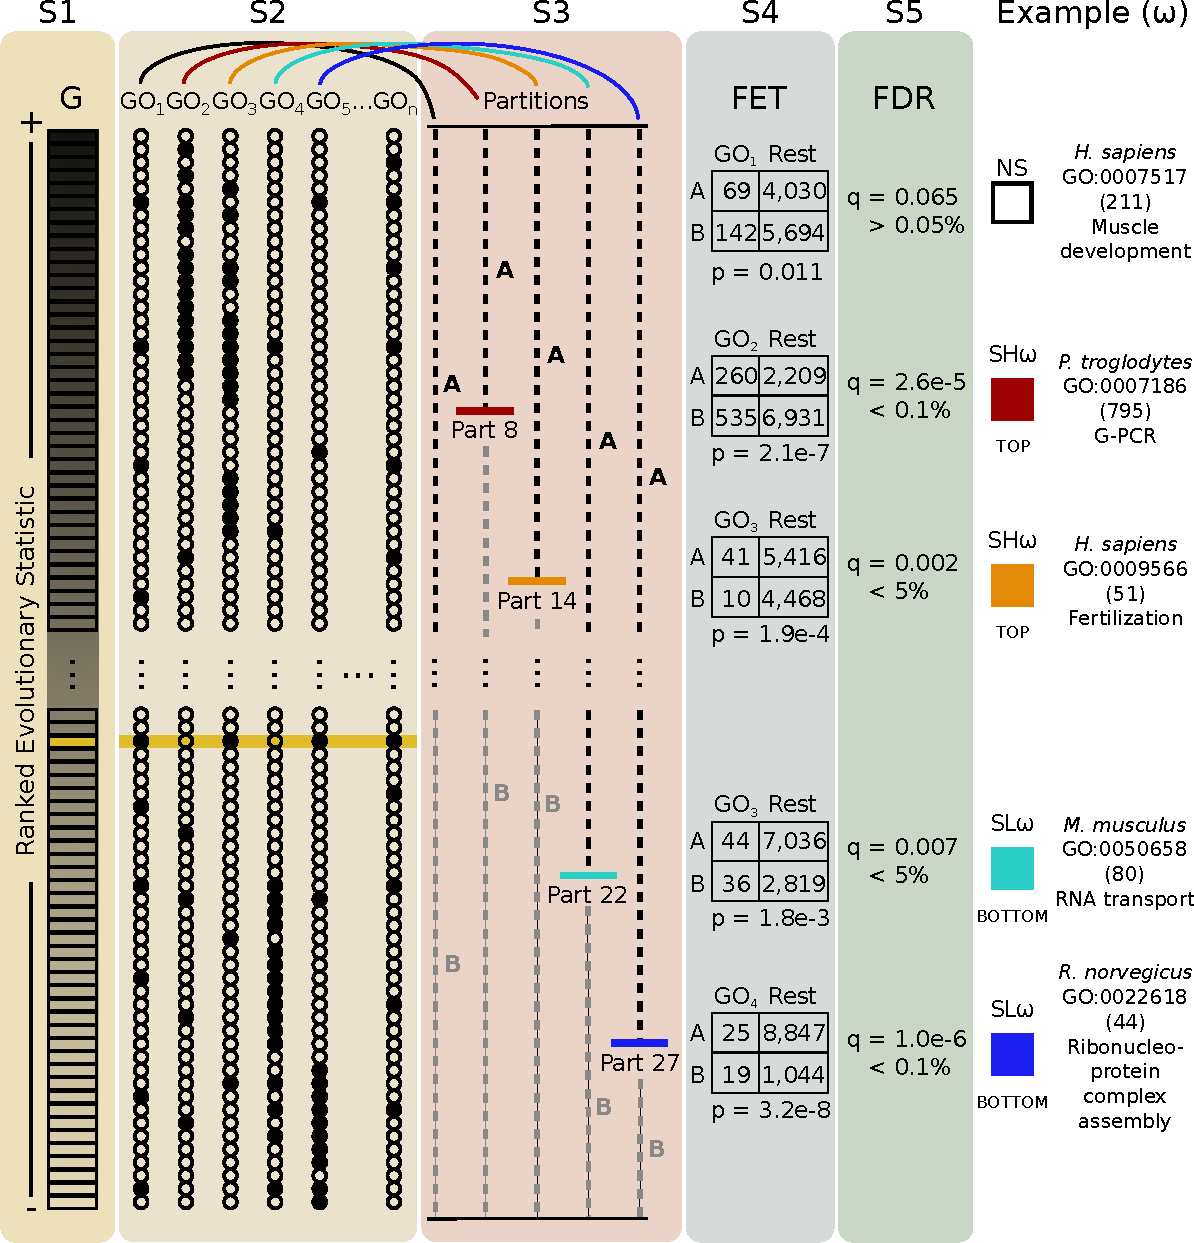
\includegraphics[width=\textwidth]{figures/material_methods/gssa_met.pdf}
\caption[Summary of the steps developed by the GSSA]{
  {\bf Summary of the steps developed by the GSSA.} \\
  GSSA can be described in a series of five steps (S1 to S5). S1: rank genes of a genome according to an evolutionary variable (e.g.: $\omega$), S2: assign functional categories, S3: partition the ranked list, S4: proceeds with a Fisher exact test for each partition, S5: adjust p-values by FDR. Colored boxes represent the final result: functional categories found to have values of $\omega$ that are a) significantly high (SH) appear in red or orange (0.1\% and 5\% FDR respectively), b) significantly low (SL) in blue and cyan (0.1\% and 5\% FDR respectively) c) not significant (NS) in white. The example shows five GO terms with significantly and NS-biased distributions of $\omega$. The number of genes annotated with the GO term is indicated in brackets. GO:0007517 is NS; although, in partition 16 in humans (not shown) its p-value was low, it was NS after FDR correction (q = 0.065). Upper (A) and lower (B) sides of the list (S3) represent both sides of the specified partition number. The remaining GO terms (GO$_2$ to GO$_5$) show the association of dark dots with values located at the top (SH$\omega$), and at the bottom (SL$\omega$) of the list (for GO$_2$-GO$_3$ and GO$_4$-GO$_5$, respectively). In examples, Fisher exact tests found the most significant p-value for partitions 8, 14, 22 and 27 for GO:0007186, GO:0009566, GO:0050658 and GO:0022618 in the chimpanzee, human, mouse and rat genomes, respectively.}
\label{fig:gssa_met}
\end{FPfigure}

Originally, 1,394/1,331 GO terms, and 199/116 KEGG pathways were analyzed in mammals/\textit{Drosophila} species, respectively. The global GO-directed acyclic graph was processed with Blast2GO \cite{Conesa2005} to extend the annotation to missing parental nodes, keeping only GO terms between levels 2 and 8 for mammals, and between levels 2 and 12 for \textit{Drosophila}. The final set of GO and KEGG terms used was also reduced to those containing at least 15 genes.

% CORRECTED rethink the presence of following 3 subsections

Some evolutionary rates presented discontinuous distributions, in particular the $\omega$ ratio. Partitioning a list by values can be pointless if this list scales from 0 to infinity. This is the case for $\omega$ values that, according to their distribution, would generate many empty partitions in between $100 < \omega < 900$. In order to partition more accurately we used the rank order instead of the direct value (see \autoref{tab:example_rank}).

\begin{table}[ht]
  \rowcolors{1}{white}{white}
  \scriptsize
  \begin{center}
    \begin{tabular}{| c | c | c || c | c |}
      \mc{1}{c}{}     & \mc{2}{c}{\textbf{Direct partitioning}} & \mc{2}{c}{\textbf{Partitioning by rank}}                                                          \\ \hline
      \textbf{Gene}   & \textbf{$\omega$ rate}                  & \textbf{Partition}                      & \textbf{rank} & \textbf{Partition}                      \\ \hline
      ENSG00000211454 & 999.0000                                & \cellcolor{black} {\color{white} A}     & 1             & \cellcolor{black} {\color{white} A}     \\ \hline
      ENSG00000169084 & 999.0000                                & \cellcolor{black} {\color{white} A}     & 1             & \cellcolor{black} {\color{white} A}     \\ \hline
      ENSG00000159433 & 999.0000                                & \cellcolor{black} {\color{white} A}     & 1             & \cellcolor{black} {\color{white} A}     \\ \hline
      ENSG00000162430 & 200.2600                                & \cellcolor{gray}  {\color{black} B}     & 4             & \cellcolor{gray}  {\color{black} B}     \\ \hline
      ENSG00000176390 & 0.2520                                  & \cellcolor{lightgray} {\color{black} C} & 5             & \cellcolor{gray}  {\color{black} B}     \\ \hline
      ENSG00000156291 & 0.0520                                  & \cellcolor{lightgray} {\color{black} C} & 6             & \cellcolor{gray}  {\color{black} C}     \\ \hline
      ENSG00000176711 & 0.0259                                  & \cellcolor{lightgray} {\color{black} C} & 7             & \cellcolor{lightgray} {\color{black} C} \\ \hline
      ENSG00000166287 & 0.0123                                  & \cellcolor{lightgray} {\color{black} C} & 8             & \cellcolor{lightgray} {\color{black} C} \\ \hline
      ENSG00000174788 & 0.0067                                  & \cellcolor{lightgray} {\color{black} C} & 9             & \cellcolor{lightgray} {\color{black} C} \\ \hline
    \end{tabular}
  \end{center}
  \caption[Comparison of partitioning strategies]{
    \textbf{Comparison of partitioning strategies.}\\
    A list of genes ranked by $\omega$, divided into three partitions (A, B and C). When values are scaled from 999 to 0, ``Direct partitioning'' would group genes within ranges of 300 resulting in few genes with $\omega$ between 300 and 600, while``Partitioning by rank'' would lead to a more continuous distribution.}
  \label{tab:example_rank}
\end{table}

\subsubsection{Methodological validation of the GSSA}
\label{sec:meth-valid-gssa}

To test possible biases attributed to the size of the functional category or the magnitude of change in evolutionary rate, we randomized the values ($\omega$, $\Delta\omega$, $dN$ and $dS$) assigned to the list of genes. Functional categories should point to the same set of genes, thus conserving all structural characteristics of the data, but suppressing the biological relevance of evolutionary rates (see  \autoref{fig:gssa_rand}).

\begin{figure}[!ht]
\centering
 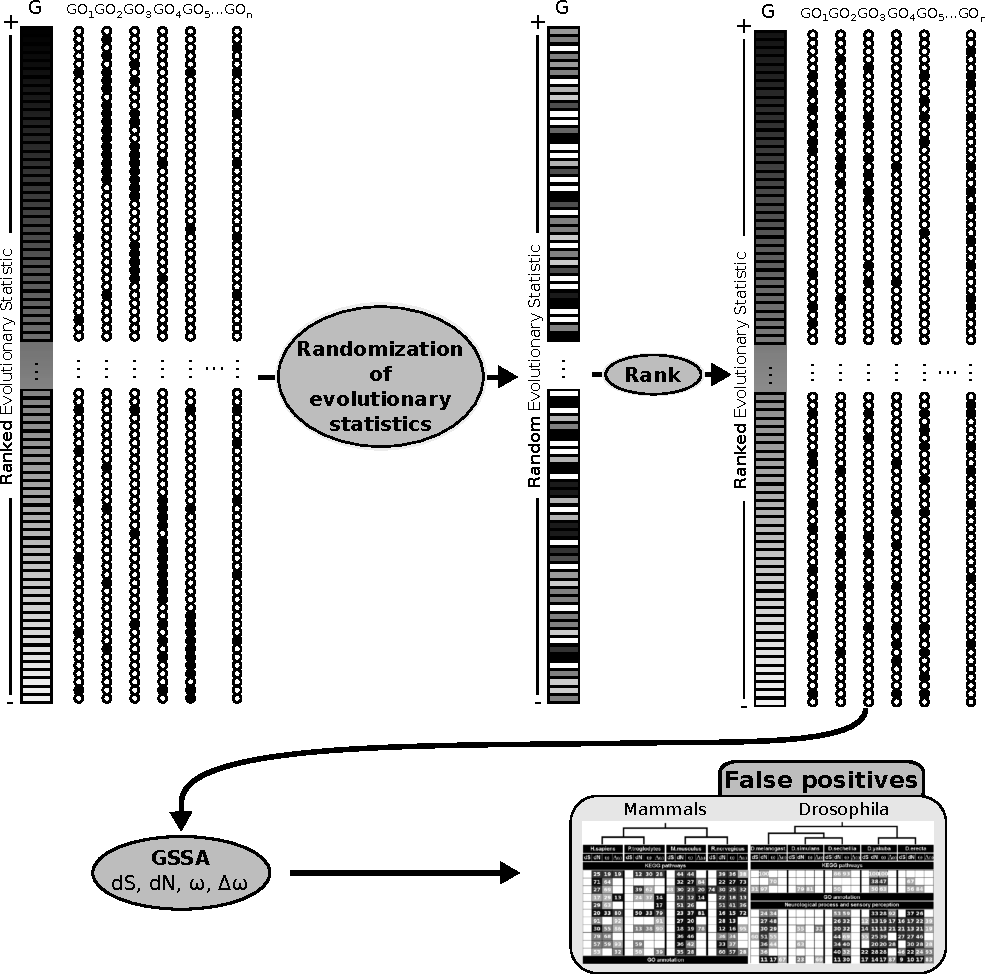
\includegraphics[width=0.95\textwidth]{figures/material_methods/random_met.pdf}
 \caption[Randomization experiment diagram]{
   {\bf Randomization experiment diagram.}\\
   The diagram shows the steps followed to test possible biases attributable to the size of functional categories. Genes are randomly re-arranged according to their evolutionary statistics. Finally, genes are ranked according to their new randomly-assigned values. The results of the enrichment analysis over this dataset are considered false positives.}
\label{fig:gssa_rand}
\end{figure}

This methodology facilitates testing of the effect of functional category sizes, and to ensure that the distribution of evolutionary rates does not affect the experiment. Each evolutionary variable was randomized 10,000 times for each species. The proportions of false positives (GSSA significant results) were plotted against the size of functional categories (from 0 to 1,500 with intervals of 20). As these proportions never attained values higher than 0.05\% FDR, we rejected the possibility that either, group sizes or rate distributions, biased the GSSA results in the dataset (see \autoref{fig:rand_result}).

\begin{PPfigure}
  \centering 
  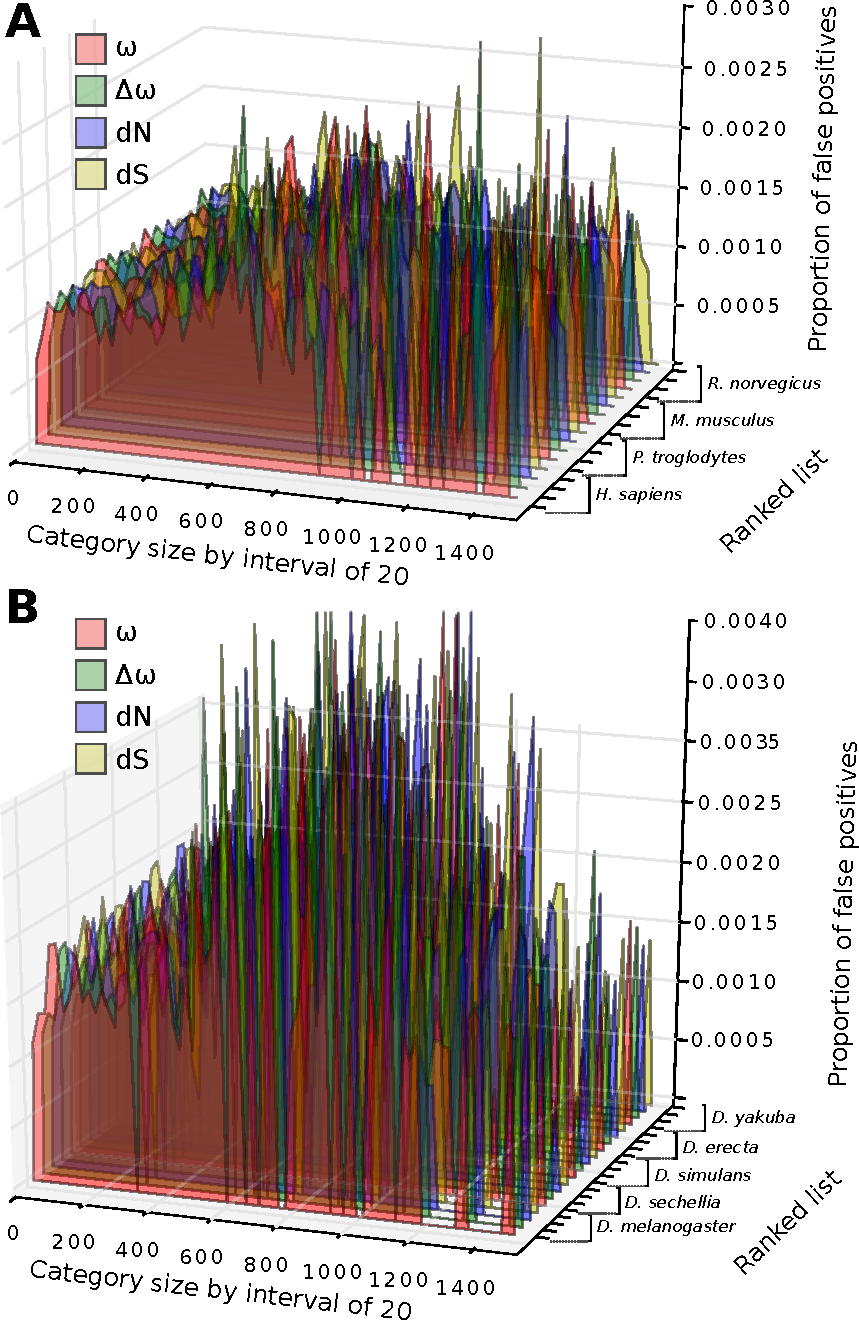
\includegraphics[height=0.9\textheight]{figures/material_methods/simulations.pdf}
  \qquad
  \caption[Randomization experiment results]{
    {\bf Randomization experiment results.}\\
    These graphics show the proportion of false positives within the results of an enrichment analysis conducted over lists of genes ranked by a shuffled evolutionary variable (see main text for details). Results are segregated into \textbf{\emph{1)}} ranges for the number of genes belonging to a functional category in order to discard the effect of category size on the proportion of false positives, and \textbf{\emph{2)}} evolutionary variables (red, green, blue and yellow for $\omega$, $\Delta\omega$, $dN$ and $dS$, respectively) and species in order to discard biases due to the specific distribution of one of the variables in a given species. Randomizations were conducted in mammals (\textbf{A}) and \textit{Drosophila} (\textbf{B}).
  }
  \label{fig:rand_result}
\end{PPfigure}

In order to better understand the results of the GSSA, a final experiment was necessary since, at this point, the possibility that results with significantly high $\omega$ were brought about only by genes under positive or relaxed selection could not be discounted.

Thus, to validate the independence of the GSSA from the effects of alternative evolutionary constraints, we simulated different selective regimes (purifying, positive and relaxed selection) using branch-site models. Here, we addressed the possibility of a variation in the representation of significant results after GSSA. The protocol diagram described in \autoref{fig:gssa_simul_pipe} shows three different areas:
\begin{figure}[H]
\centering 
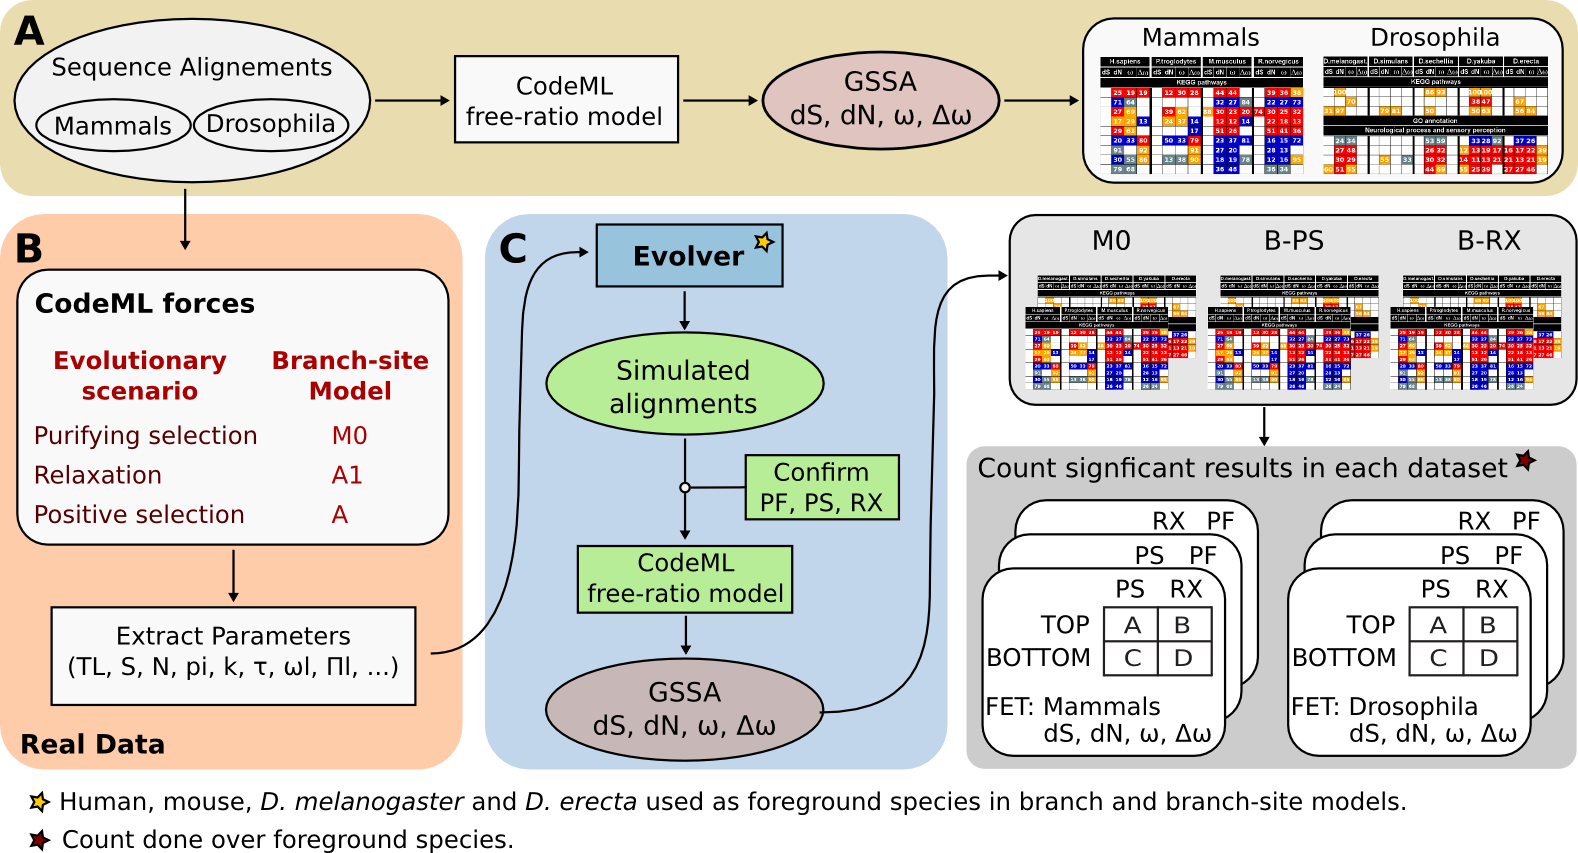
\includegraphics[width=\textwidth]{figures/material_methods/simulations_met.png}
\caption[Evolutionary and statistical simulation of GSSA]{
  {\bf Evolutionary and statistical simulation of GSSA.}\\
  The protocol diagram shows the steps taken along three different analytical spaces, the real data, the simulated data and the testing block. See main text for a complete explanation.}
\label{fig:gssa_simul_pipe}
\end{figure}
\begin{itemize}
\item \textbf{Real Data}: the light yellow area (\textbf{A}) describes the steps of the GSSA. The orange area (\textbf{B}) describes the use of the CodeML program from PAML package \cite{Yang2007} to extract from the original set of sequences all evolutionary parameters needed to simulate new sequences under purifying selection (PF), positive selection (PS) or relaxation of selective constraints (RX) according to branch-site models. Human, mouse, \textit{D. erecta} and \textit{D. melanogaster} were used as foreground species in the corresponding models.
  
\item \textbf{Simulated Data}: in the light blue area (\textbf{C}), the Evolver program (also from the PAML package \cite{Yang2007}) simulates sequences evolving under the given parameters (codon frequencies and branch lengths) estimated from the empirical data. We checked the desired characteristics of PS and RX on the set of the simulated sequences \autoref{tab:psg_simul}. The evolutionary variables ($dS$, $dN$, $\omega$ and $\Delta\omega$) were estimated from simulated sequences using a free-ratio branch model. The complete GSSA protocol was applied over the simulated data.
  
\item \textbf{Testing simulation}: the last part of the diagram represents the calculation of the odd-ratios corresponding to a classification of the GSSA results over all datasets. Significant categories are counted for the contingency tables, with either SH$\omega$ or SL$\omega$. and belonging to two of the three simulated selective regimes (PS, RX and PF). Odd-ratio values represent the association between different selective regimes, simulated according to their proportions of SH and SL functional categories. Statistical contributions of the simulated regimes (PS, RX and PF) to the GSSA results were tested by comparing log odd-ratios with a t-test (results in \autoref{tab:prop_signif}).
\end{itemize}

\rowcolors{1}{lightgray}{white}
\begin{table}[htbp]
  \scriptsize
  \centering
    \begin{tabular}{l r r r r r r}
      \mc{1}{l}{}              & \mc{ 2}{c}{PS}    & \mc{ 2}{c}{RX}    & \mc{ 2}{c}{PF}                                                                \\ \hline
      \mc{1}{l}{}              & \mc{1}{c}{ PSG} & \mc{1}{c}{ RXG} & \mc{1}{c}{ PSG} & \mc{1}{c}{ RXG} & \mc{1}{c}{ PSG} & \mc{1}{c}{ RXG} \\ \hline
      \textit{H. sapiens}      & 658               & 1640              & 11                & 1939              & 0                 & 1                 \\
      \textit{M. musculus}     & 1500              & 954               & 14                & 1565              & 1                 & 0                 \\
      \textit{D. melanogaster} & 736               & 630               & 25                & 1104              & 0                 & 0                 \\
      \textit{D. erecta}       & 778               & 1292              & 26                & 1713              & 2                 & 1                 \\ \hline
    \end{tabular}
    \caption[Number of genes under positive and relaxed selection in each of the simulated evolutionary scenarios]{
      \textbf{Number of genes under positive and relaxed selection in each of the simulated evolutionary scenarios.}}
  \label{tab:psg_simul}
\end{table}

The results showed that, in spite of the alternative evolutionary scenarios, no significant differences were found between log odd-ratio distributions (p$<$0.05). The average effect of PF and RX/PS is a proportional decrease and increase of the mean $\omega$ value on sequences, respectively. This change has minor effects (if any) on the relative position of genes in the ranked list of genes of the genomes. Accordingly, since no net differences were produced after ranking genes, no significant differences are expected after the t-test (PS-RX: p= 0.99, PS-PF: p= 0.45, and RX-PF: p= 0.46).

The fact that, basically, the same number of significant results was observed in each evolutionary scenario confirmed this prediction \autoref{tab:prop_signif}. We conclude that none of the simulated selective regimes produce significant differences or biases in the GSSA of $\omega$ values.

\begin{table}
  \begin{center}
    \scriptsize
    \begin{tabular}{l c c c}
                     & \textbf{PS} & \textbf{RX} & \textbf{PF} \\ \hline
         \textbf{PS} & ---         & 92.50\%     & 98.50\%     \\
         \textbf{RX} & 91.10\%     & ---         & 99.00\%     \\
         \textbf{PF} & 88.90\%     & 90.60\%     & ---         \\ \hline
    \end{tabular}
  \end{center}
  \caption[Proportion of significant functional categories coinciding in two simulated evolutionary scenarios]{
    \textbf{Proportion of significant functional categories coinciding for two simulated evolutionary scenario}, or retaining identical signs of odd-ratios under a different evolutionary scenario.}
  \label{tab:prop_signif}
\end{table}


%%% Local Variables: 
%%% mode: latex
%%% TeX-master: "../../thesis_main"
%%% End: 
